\chapter{シミュレーションの結果と考察}
%数値の取り直し,プロットエリアの見直しと枠をつける
%考察書く

本章では,前章で述べた同時送信フラッディングにおけるホスト選択手法をシミュレーションによって評価した結果について述べる.

\section{シミュレーション諸元}
媒介中心性と次数中心性はRのパッケージigraph内の関数betweennessと関数degreeで求めた.次数中心性と媒介中心性,それぞれの上位10\%ノードをホストノードにした場合とランダムに選んだ10\%ノードをホストノードに選んだときの比較を行う.
シミュレーションには,統計解析向けのプログラム言語であるR~\cite{R}を用いた.Rは機械学習やネットワーク分析のパッケージも豊富である.本研究では主にRのパッケージの一つであるigraphを使用した.
デフォルトではコアを1つしか使わない設定で,シミュレーションに時間がかかってしまうため,parallelパッケージとSNOWパッケージを使用し,並列化することでシミュレーション時間の短縮を図った.使用したRのバージョンやパッケージを表\ref{tab:sim_info}に示す.

\begin{table}[H]
\centering
  \caption{シミュレーション環境}
  \begin{tabular}{c|c} \hline\hline
    項目 & 内容  \\ \hline 
    package& parallel doSNOW  xlsx dplyr igraph\\
    R & R x64 3.6.1\\\hline\hline
  \end{tabular}
  \label{tab:sim_info}
\end{table}
%パッケージ説明
doSNOWパッケージとparallelパッケージは並列化に用いた.

シミュレーションに用いたパラメータは表\ref{tab:para_info}である.
\begin{table}[H]
\centering
  \caption{シミュレーション環境}
  \begin{tabular}{c|c|c} \hline\hline 
    項目 & 変数& 値  \\ \hline 
    ノード数& N & 50,100\\
    位置範囲& range & 250\\
    ホストノード数& host & 5,10\\
    到達範囲 & reach &20,30,40,50\\\hline\hline
  \end{tabular}
  \label{tab:para_info}
\end{table}

まず,250を上限としてランダムに生成した乱数を行列d(N,2)に代入し,ノードのxy座標とした.図\ref{fig:plotnode}は,これをプロットした一例である.x軸のd[,1]は行列dの1行目,y軸のd[,2]は行列dの2行目を表しており,これがx座標とy座標に対応している.単位は\si{\meter}である.


\begin{figure}[H]
  \centering
  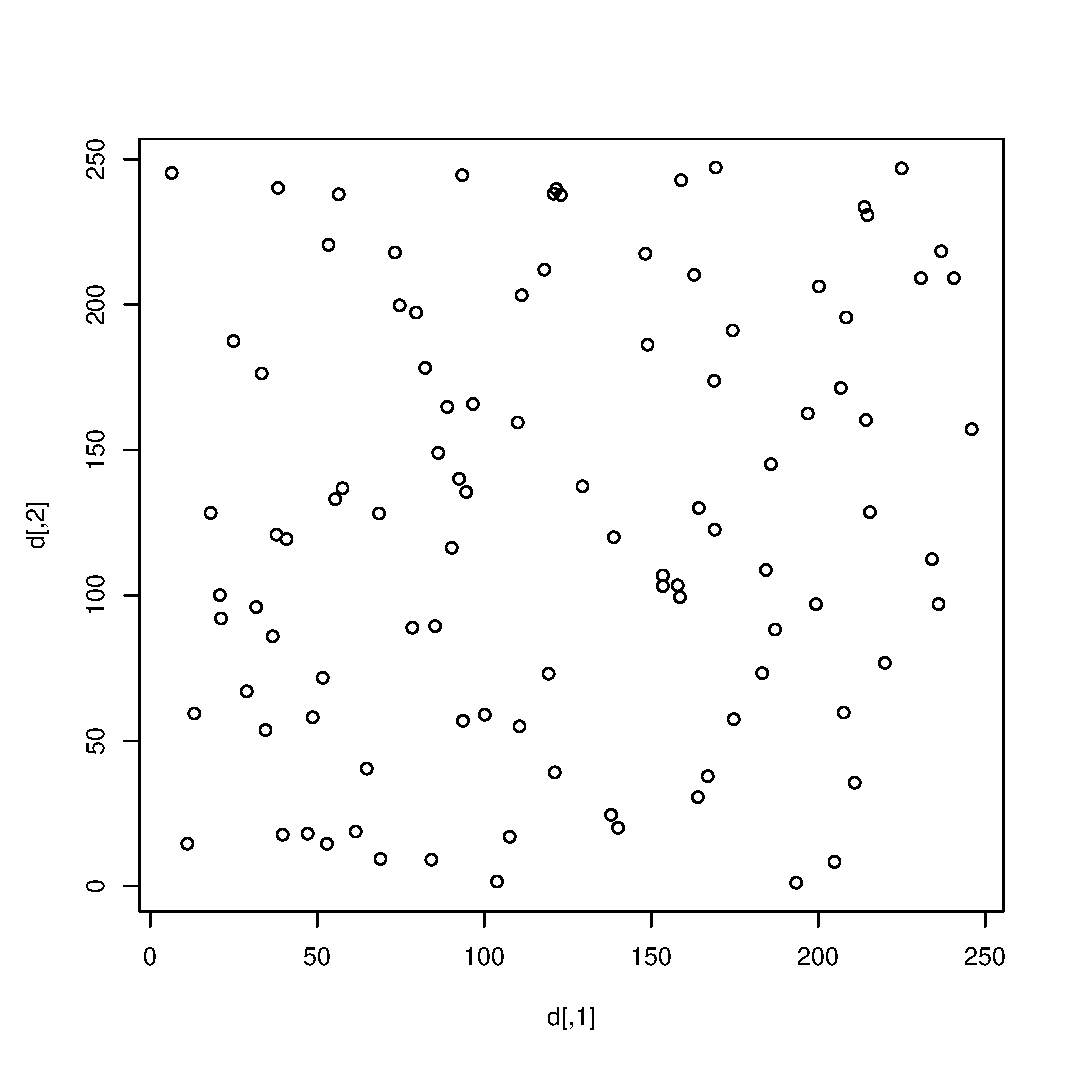
\includegraphics[width=0.8\textwidth]{figures/plotnode.eps}
  \caption{ノード位置}
  \label{fig:plotnode}
\end{figure}

その後,方法1は距離をしきい値としてその範囲内であれば完全に到達するという状況で,方法2は距離に反比例して下がる到達確率によって到達判定を行い,ネットワークグラフを作成した.生成されたネットワークグラフの一例を図\ref{fig:plotgraph}に示す.
\begin{figure}[H]
  \centering
  \includegraphics[width=0.8\textwidth]{figures/plotg.png}
  \caption{図\ref{fig:plotnode}から生成したネットワークグラフ}
  \label{fig:plotgraph}
\end{figure}

それぞれにおいて媒介中心性と次数中心性の上位10\%ノードをホストノードとした際の最短経路長平均とInf数をダイクストラ法によって求めた.比較対象は,全ノードの10\%のノードをランダムに選出した際の最短経路長平均とInf数である.
また,ノードの配置による影響を除外するため,方法1,2ともに上記の過程をシード値を変更して1万回行った.

%%%%%%%%%%%%%%%%%%%%%%%%%方法1開始%%%%%%%%%%%%%%%%%%%%%%%%%%%%%%%%%%

\section{方法1:距離による到達判定}
方法1は到達距離を設定し,その範囲内であれば通信が100\%可能であるという状況を想定したシミュレーションである.媒介中心性と次数中心性で上位10\%ノードをホストノードとした時の最短経路長平均を表\ref{tab:1_spl_bet}に示す.なお,50ノードで到達範囲を20とした際,従来手法では,NAという値が含まれてしまい,最短経路長平均が求まらなかった.ノード密度が低いことと,到達範囲が狭いことで,通信が成立しなかったためと思われる.表にはNAを除外した値を載せている.そのためグラフ上は20\si{\meter}において平均最短経路長が短く出ているが,実際は最短経路長平均が存在しない(すべてのノードがつながっていない)状態を含んでいる.

\begin{comment}
\begin{table}[H]
\centering
\caption{方法1の平均最短経路長}
\scalebox{0.55}[0.55]{
  \begin{tabular}{c|c|c|c|c|c|c} \hline\hline
     到達距離 [\si{\meter}] & 50従来 [ホップ] &50媒介 [ホップ]&50次数 [ホップ] &100従来 [ホップ]& 100媒介 [ホップ]& 100次数 [ホップ]\\ \hline 
    20 & 1.343 & 1.346 & 1.277& 2.275 & 2.420 & 1.993\\
    30 & 2.161 & 2.123 & 1.858 & 5.295 & 4.487 & 4.497\\
    40 & 3.386 & 2.903 & 2.778 & 4.243 & 3.523 & 3.572\\
    50 & 3.451 & 2.824 & 2.780 & 3.196 & 2.691 & 2.697\\ \hline\hline
  \end{tabular}
  }
\label{tab:1_spl_bet}
\end{table}
\end{comment}

\begin{table}[H]
\centering
\caption{方法1の平均最短経路長}
\scalebox{1}[1]{
  \begin{tabular}{c|c|c|c|c} \hline\hline
 & 20 [\si{\meter}] & 30 [\si{\meter}] & 40 [\si{\meter}] &50 [\si{\meter}]\\ \hline
50従来 & 1.343 & 2.161 & 3.386 & 3.451 \\
50媒介 & 1.346 & 2.123 & 2.903 & 2.824 \\
50次数 & 1.277 & 1.858 & 2.778 & 2.78 \\ 
100従来 & 2.275 & 5.295 & 4.243 & 3.196 \\ 
100媒介 & 2.42 & 4.487 & 3.523 & 2.691 \\ 
100次数 & 1.993 & 4.497 & 3.572 & 2.697 \\ \hline\hline
  \end{tabular}
  }
\label{tab:1_spl_bet}
\end{table}

表\ref{tab:1_spl_bet}の内容を手法ごとにプロットしたものを図\ref{fig:1hopall}に示す.

\begin{figure}[H]
  \centering
  \includegraphics[width=1.05\textwidth]{figures/1spl.pdf}
  \caption{到達距離ごとの方法1の最短経路長平均}
  \label{fig:1hopall}
\end{figure}

いずれの場合においてもランダムに選んだ10\%ノードをホストノードとした従来手法よりもホスト選択を行った方が最短経路長平均が短い.また,媒介中心性でホスト選択したときと次数中心性でホスト選択したときを比較すると,ノード数に関わらず次数中心性の方がよい.しかし,到達距離が大きくなるにつれ2つの差は縮まり,ノードが50・100いずれの場合でも到達距離が50\si{\meter}のときはあまり差が見られない.

ここで50ノードと100ノードにおける次数中心性と媒介中心性の分布を図\ref{fig:50100bg}に示す.上2つのヒストグラムが50ノード,下2つが100ノードで,左側の2つのヒストグラムが媒介中心性の分布,右2つが次数中心性の分布を示している.

\begin{figure}[H]
  \centering
  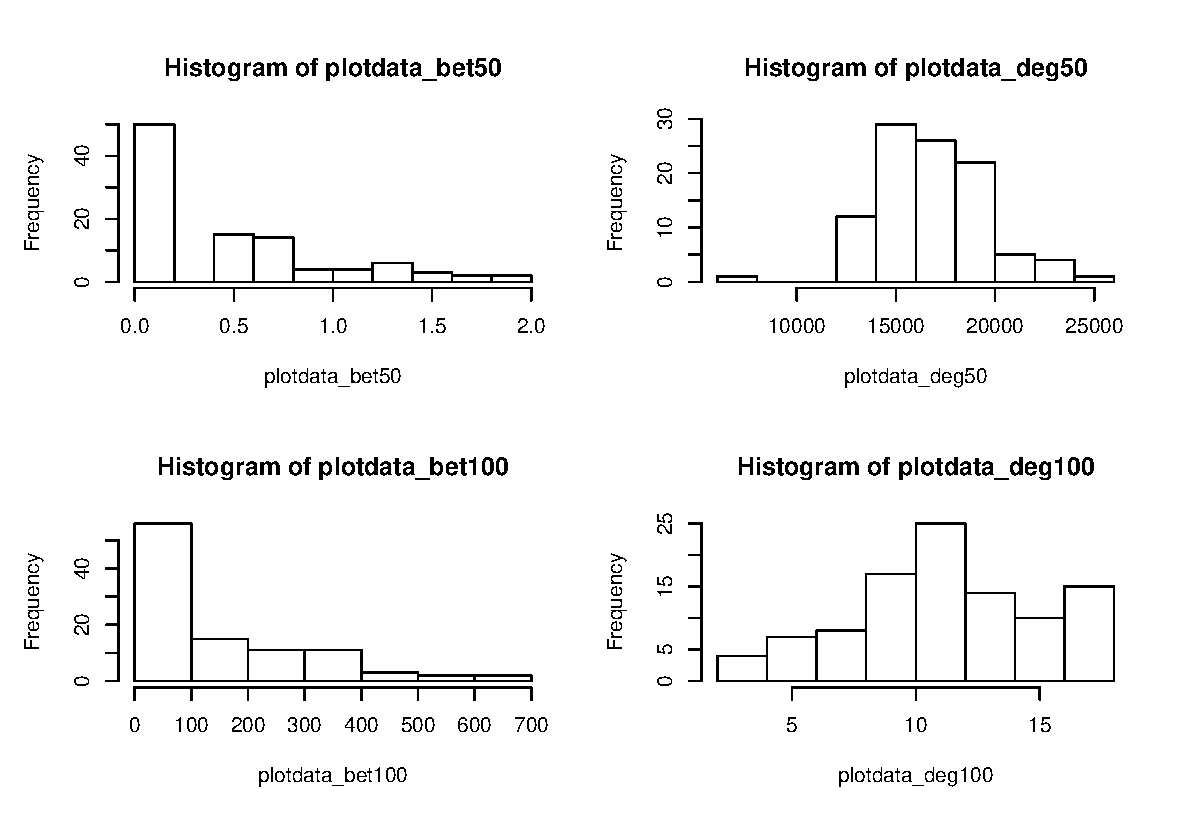
\includegraphics[width=1\textwidth]{figures/50100bg.eps}
  \caption{ノード数による媒介中心性と次数中心性の分布の違い}
  \label{fig:50100bg}
\end{figure}

ノード数によって次数中心性と媒介中心性の値の桁が大きく変わることがわかる.ノードの密度が高い50ノードにおいては,次数中心性が大きくなるのは自明であり,次数中心性がノードの密度に大きく影響されることがわかる.また,到達範囲が広がるということは通信可能範囲内のノードが増えるということでこれも間接的にノードの密度が大きくなっているといえる.
本研究では,次数中心性による選択の方が最短経路長平均が短くなったが,さらにノード数を増やし,ノード密度が大きくなる場合は,媒介中心性の方が最短経路長平均が短くなると推測される.
また,同時送信フラッディングの,ノード過密時は性能が下がるという特徴を考慮すると,ノードが密なときに性能がいい次数中心性によるホスト選択より媒介中心性によるホスト選択の方が同時送信フラッディングに適しているといえる.

%%%%%%%%%%%%%%%%%%%%%%↑方法1最短経路長平均%%%%%%%%%%%%%%%%%%%%%%%%%%

%%%%%%%%%%%%%%%%%%%%%%%%%%%↓方法1Inf数%%%%%%%%%%%%%%%%%%%%%%%%%%

\begin{comment}

\begin{table}[H]
\centering
  \caption{方法1のInf数}
\scalebox{0.55}[0.55]{
  \begin{tabular}{c|c|c|c|c|c|c} \hline\hline
    到達距離 [\si{\meter}] & 50従来 [個] &50媒介 [個]&50次数 [個] &100従来 [個]& 100媒介 [個]& 100次数 [個]\\ \hline 
    20 & 116,735,452(93.4\%) & 111,497,510(89.2\%) & 111,158,504(88.9\%) & 933,612,885(93.4\%) & 870,218,229(87.0\%) & 888,797,275(88.9\%)\\
    30 & 107,704,036(86.2\%) & 95,797,648(76.6\%)  & 98,417,647(78.7\%) & 641,037,650(64.1\%) & 536,432,013(53.6\%) & 578,549,885(57.9\%)\\
    40 & 81,753,752(65.4\%) & 67,507,031(54.0\%)   & 71,600,767(57.3\%) & 373,913,223 (37.4\%)& 339,721,118(34.0\%) & 362,988,951(36.3\%)\\
    50 & 52,258,853 (41.8\%)& 44,334,309(35.5\%)& 47,604,897(38.1\%) & 296,649,201(29.7\%) & 258,705,947(25.9\%) & 290,858,488(29.1\%)\\ \hline\hline
  \end{tabular}
  }
  \label{tab:1_inf}
\end{table}
\end{comment}

\begin{table}[H]
\centering
  \caption{方法1のInf数}
\scalebox{1}[1]{
  \begin{tabular}{c|c|c|c|c} \hline\hline
 &20 [\si{\meter}] & 30 [\si{\meter}] & 40 [\si{\meter}] & 50 [\si{\meter}] \\ \hline
50従来 & 93.4 & 86.2 & 65.4 & 42 \\ 
50媒介 & 89.2 & 76.7 & 54 & 35.5 \\ 
50次数 & 88.9 & 78.7 & 57.3 & 38.1 \\ 
100従来 & 93.4 & 64.1 & 37.4 & 29.7 \\ 
100媒介 & 87 & 53.6 & 34 & 25.9 \\ 
100次数 & 88.9 & 57.9 & 36.3 & 29.1 \\ \hline\hline
  \end{tabular}
  }
  \label{tab:1_inf}
\end{table}







\begin{figure}[H]
  \centering
  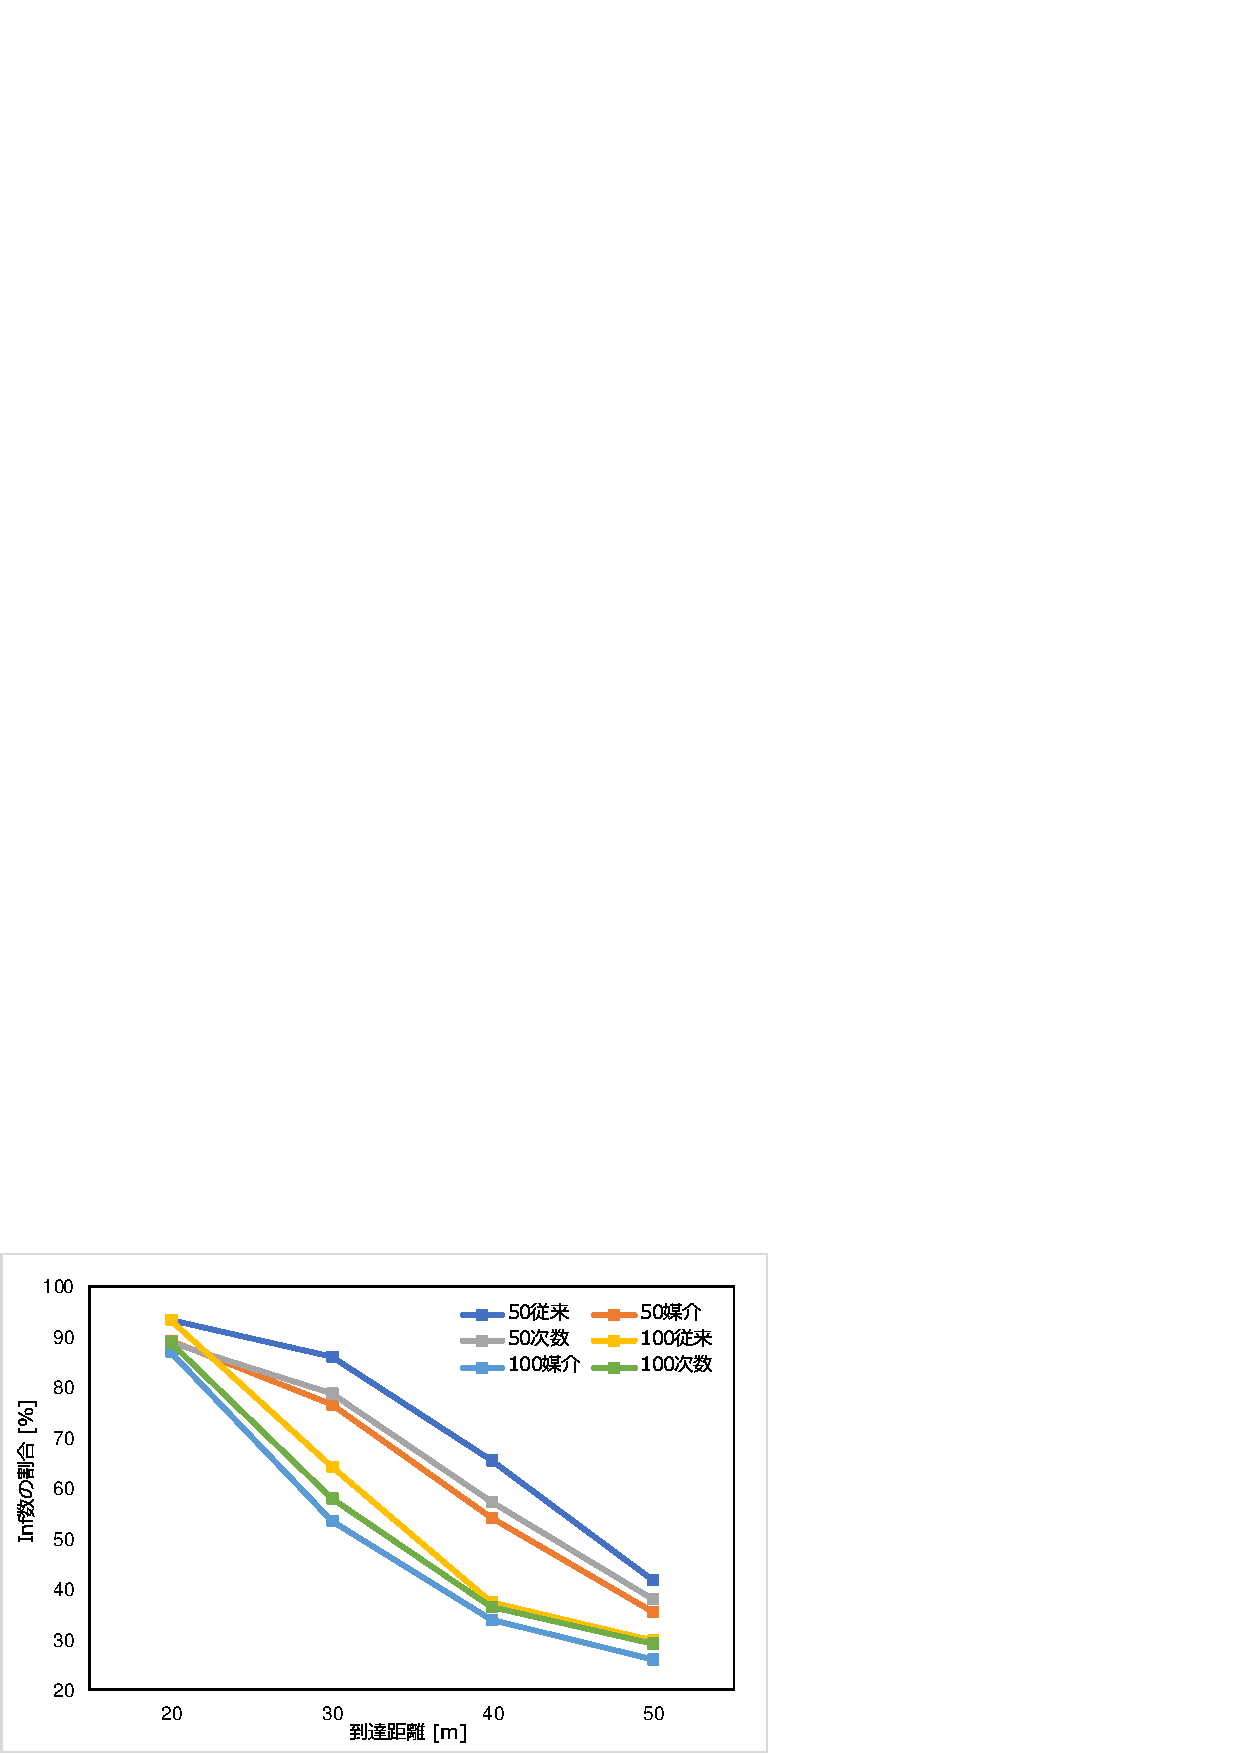
\includegraphics[width=1.05\textwidth]{figures/1Inf.pdf}
  \caption{到達距離ごとの方法1のInf数の割合}
  \label{fig:1Infall}
\end{figure}
方法1におけるInf数はノード数が50,到達範囲が20\si{\meter}のときのみ次数中心性がわずかによく,それ以外においては媒介中心性がよいことがわかった.先述のように50ノードで到達範囲が20\si{\meter}のときは例外的な値を含んでいるため,ここでは除外する.
また,到達距離に反比例してInf数の割合が下がることが見て取れるが,これはノード密度が大きくなるためだと考えられる.
また,100ノードで到達距離が50\si{\meter}のときは,従来手法と提案手法の差が小さいこともわかる.ノード密度が大きい場合は,ホストノードをランダムに選んだ場合でも,ネットワーク分断の可能性が小さくなることが示唆されている.一方,50ノードにおいては従来手法と提案手法の差は大きく,ノード密度が小さい状況においてはホストノードを中心性によって選出することの有効性が確認できた.
%%%%%%%%%%%%%%%%%%%%%%%%%方法2開始%%%%%%%%%%%%%%%%%%%%%%%%%%%%%%%%%%

\section{方法2:確率による到達判定}
次にノイズ等の影響により通信が失敗した状況を想定し,距離の2乗に反比例する確率による到達判定を行った.方法1では設定した到達距離内であれば100\%通信が可能であるとしてシミュレーションを行ったが,方法2においては近くても失敗する可能性があり,遠くても成功する可能性があるという状態でシミュレーションを行った.

\begin{table}[H]
    \centering
  \caption{方法2の平均最短経路長}
\scalebox{0.5}[0.5]{
  \begin{tabular}{c|c|c|c|c|c} \hline\hline
       50従来 [ホップ] &50提案(媒介) [ホップ]&50提案(次数) [ホップ] &100従来 [ホップ]& 100提案(媒介) [ホップ]& 100提案(次数) [ホップ] \\ \hline 
       2.086 & 1.792 & 1.740 & 2.001 & 1.756 & 1.733\\ \hline\hline
  \end{tabular}
  }
  \label{tab:2_spl}
\end{table}


\begin{figure}[H]
  \centering
  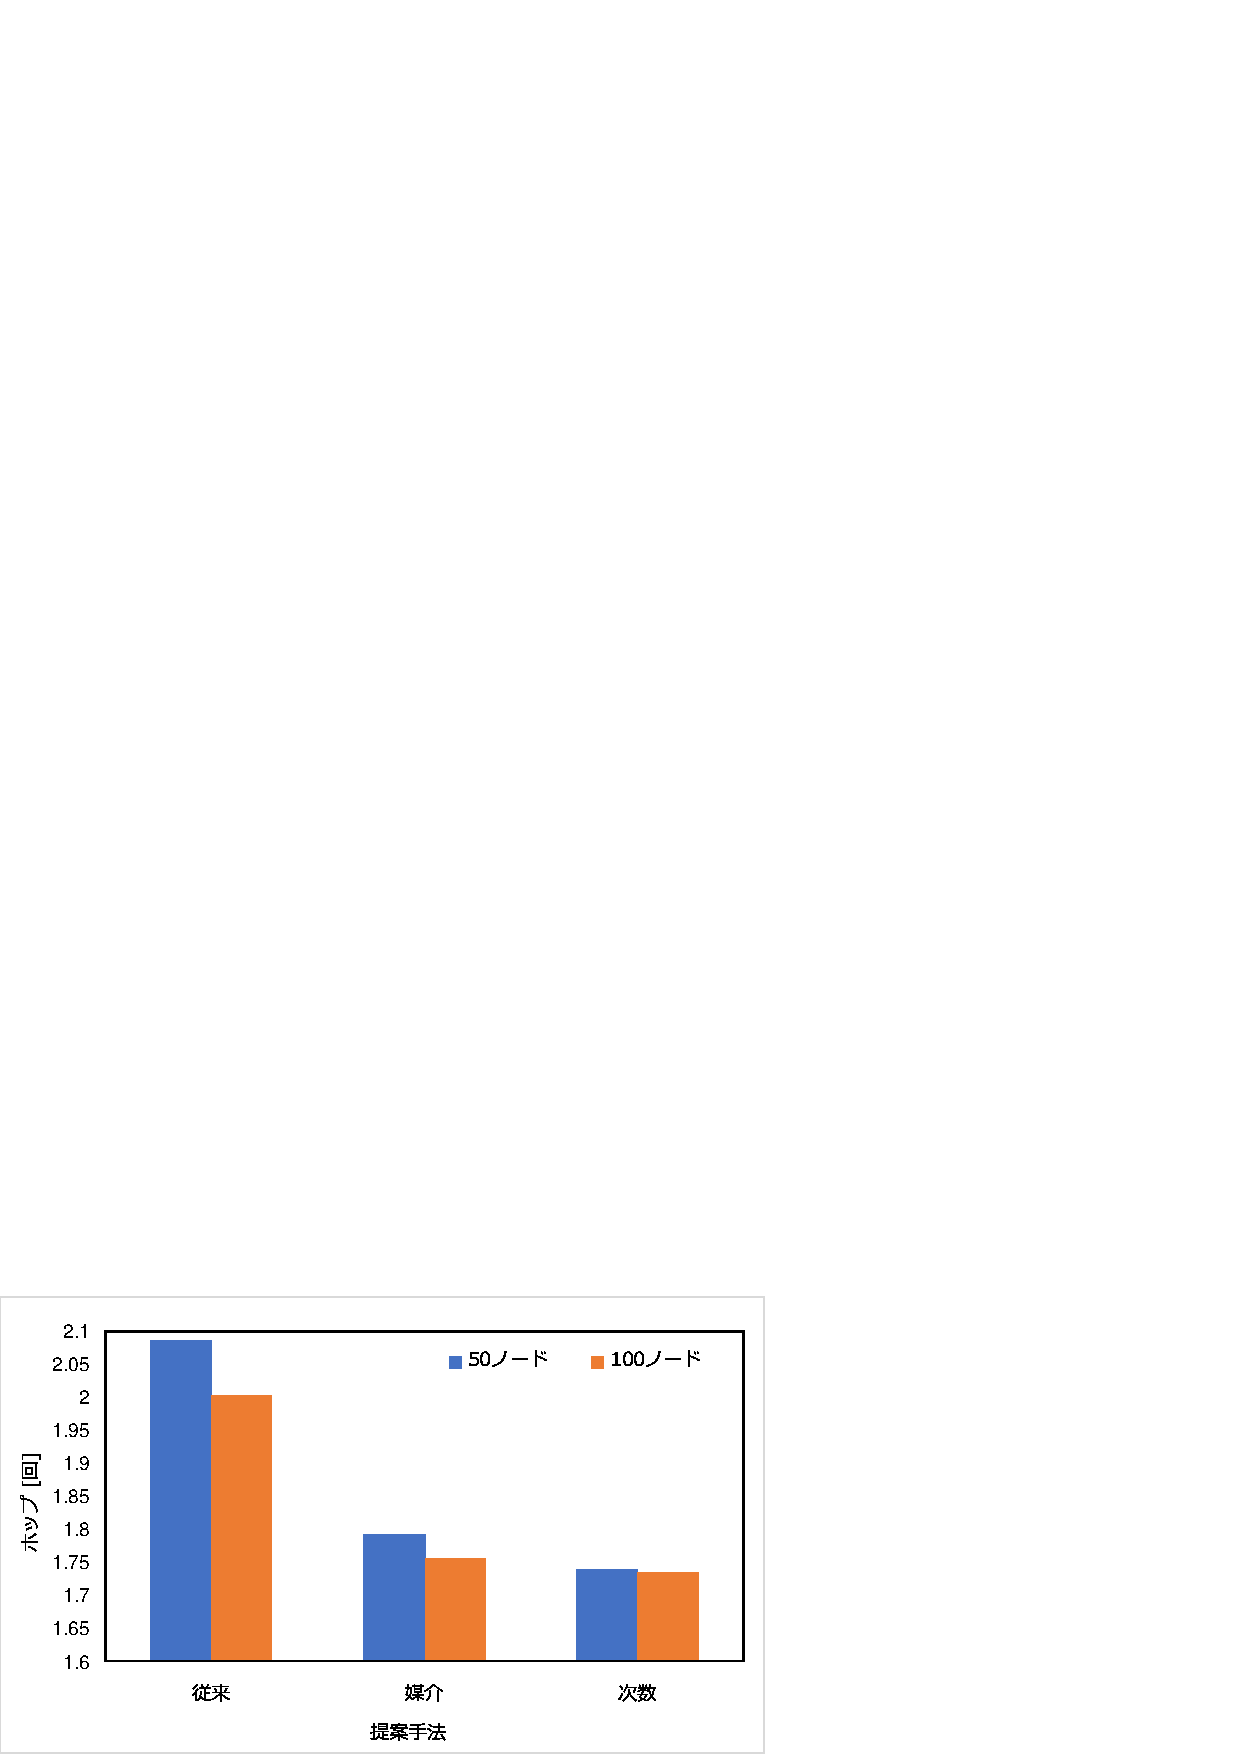
\includegraphics[width=1\textwidth]{figures/2hop.pdf}
    \vspace{-20mm}
  \caption{方法2の最短経路長平均}   
  \label{fig:2hop}
\end{figure}

いずれの提案手法も従来手法に比べて最短経路長平均が小さく,従来のリストによるラウンドロビン方式のホスト選択より,到達性を考慮してホスト選択を行った方がよいということがわかった.
また,媒介中心性でホスト選択した場合と,次数中心性でホスト選択した場合では,ノード数に関係なく次数中心性による選択の方がよい結果となった.


\begin{table}[H]
    \centering
  \caption{方法2のInf数}
\scalebox{0.55}[0.55]{
  \begin{tabular}{c|c|c|c|c|c|c} \hline\hline
       50従来 [個] &50媒介 [個]&50次数 [個] &100従来 [個]& 100媒介 [個]& 100次数 [個] \\ \hline 
      22,467,967(18.0\%) & 16,491,898(13.2\%) &19,554,978(15.6\%)& 130,496,056(13.0\%) & 83,183,195(8.32\%)& 100,239,883(10.0\%) \\ \hline\hline
  \end{tabular}
  }
  \label{tab:2_inf}
\end{table}

\begin{figure}[H]
  \centering
  \includegraphics[width=1\textwidth]{figures/2inf.pdf}
  \label{fig:2Inf}
      \vspace{-20mm}
    \caption{方法2のInf数の割合}
\end{figure}

一方,Infの割合においては,ノード数が50のときでも100のときでも媒介中心性によるホスト選択が最もよい結果となった.
また方法1,2ともに50ノードのInf数が多いのは,ノードの密度が小さいことで繋がっている辺が少なくなるからであり,直感的にも納得のいく結果となった.


%%%%%%%%%%%%%%%%%%%%%%%%%グラフ%%%%%%%%%%%%%%%%%%%%%%%%%%%%%%%%%%

\section{全結果}
本研究のシミュレーションにおける全結果の累積分布関数プロットとヒストグラムを図\ref{fig:1_50_30}から図\ref{fig:2_100}に示す.
\begin{landscape}
\begin{figure}[H]
  \centering
  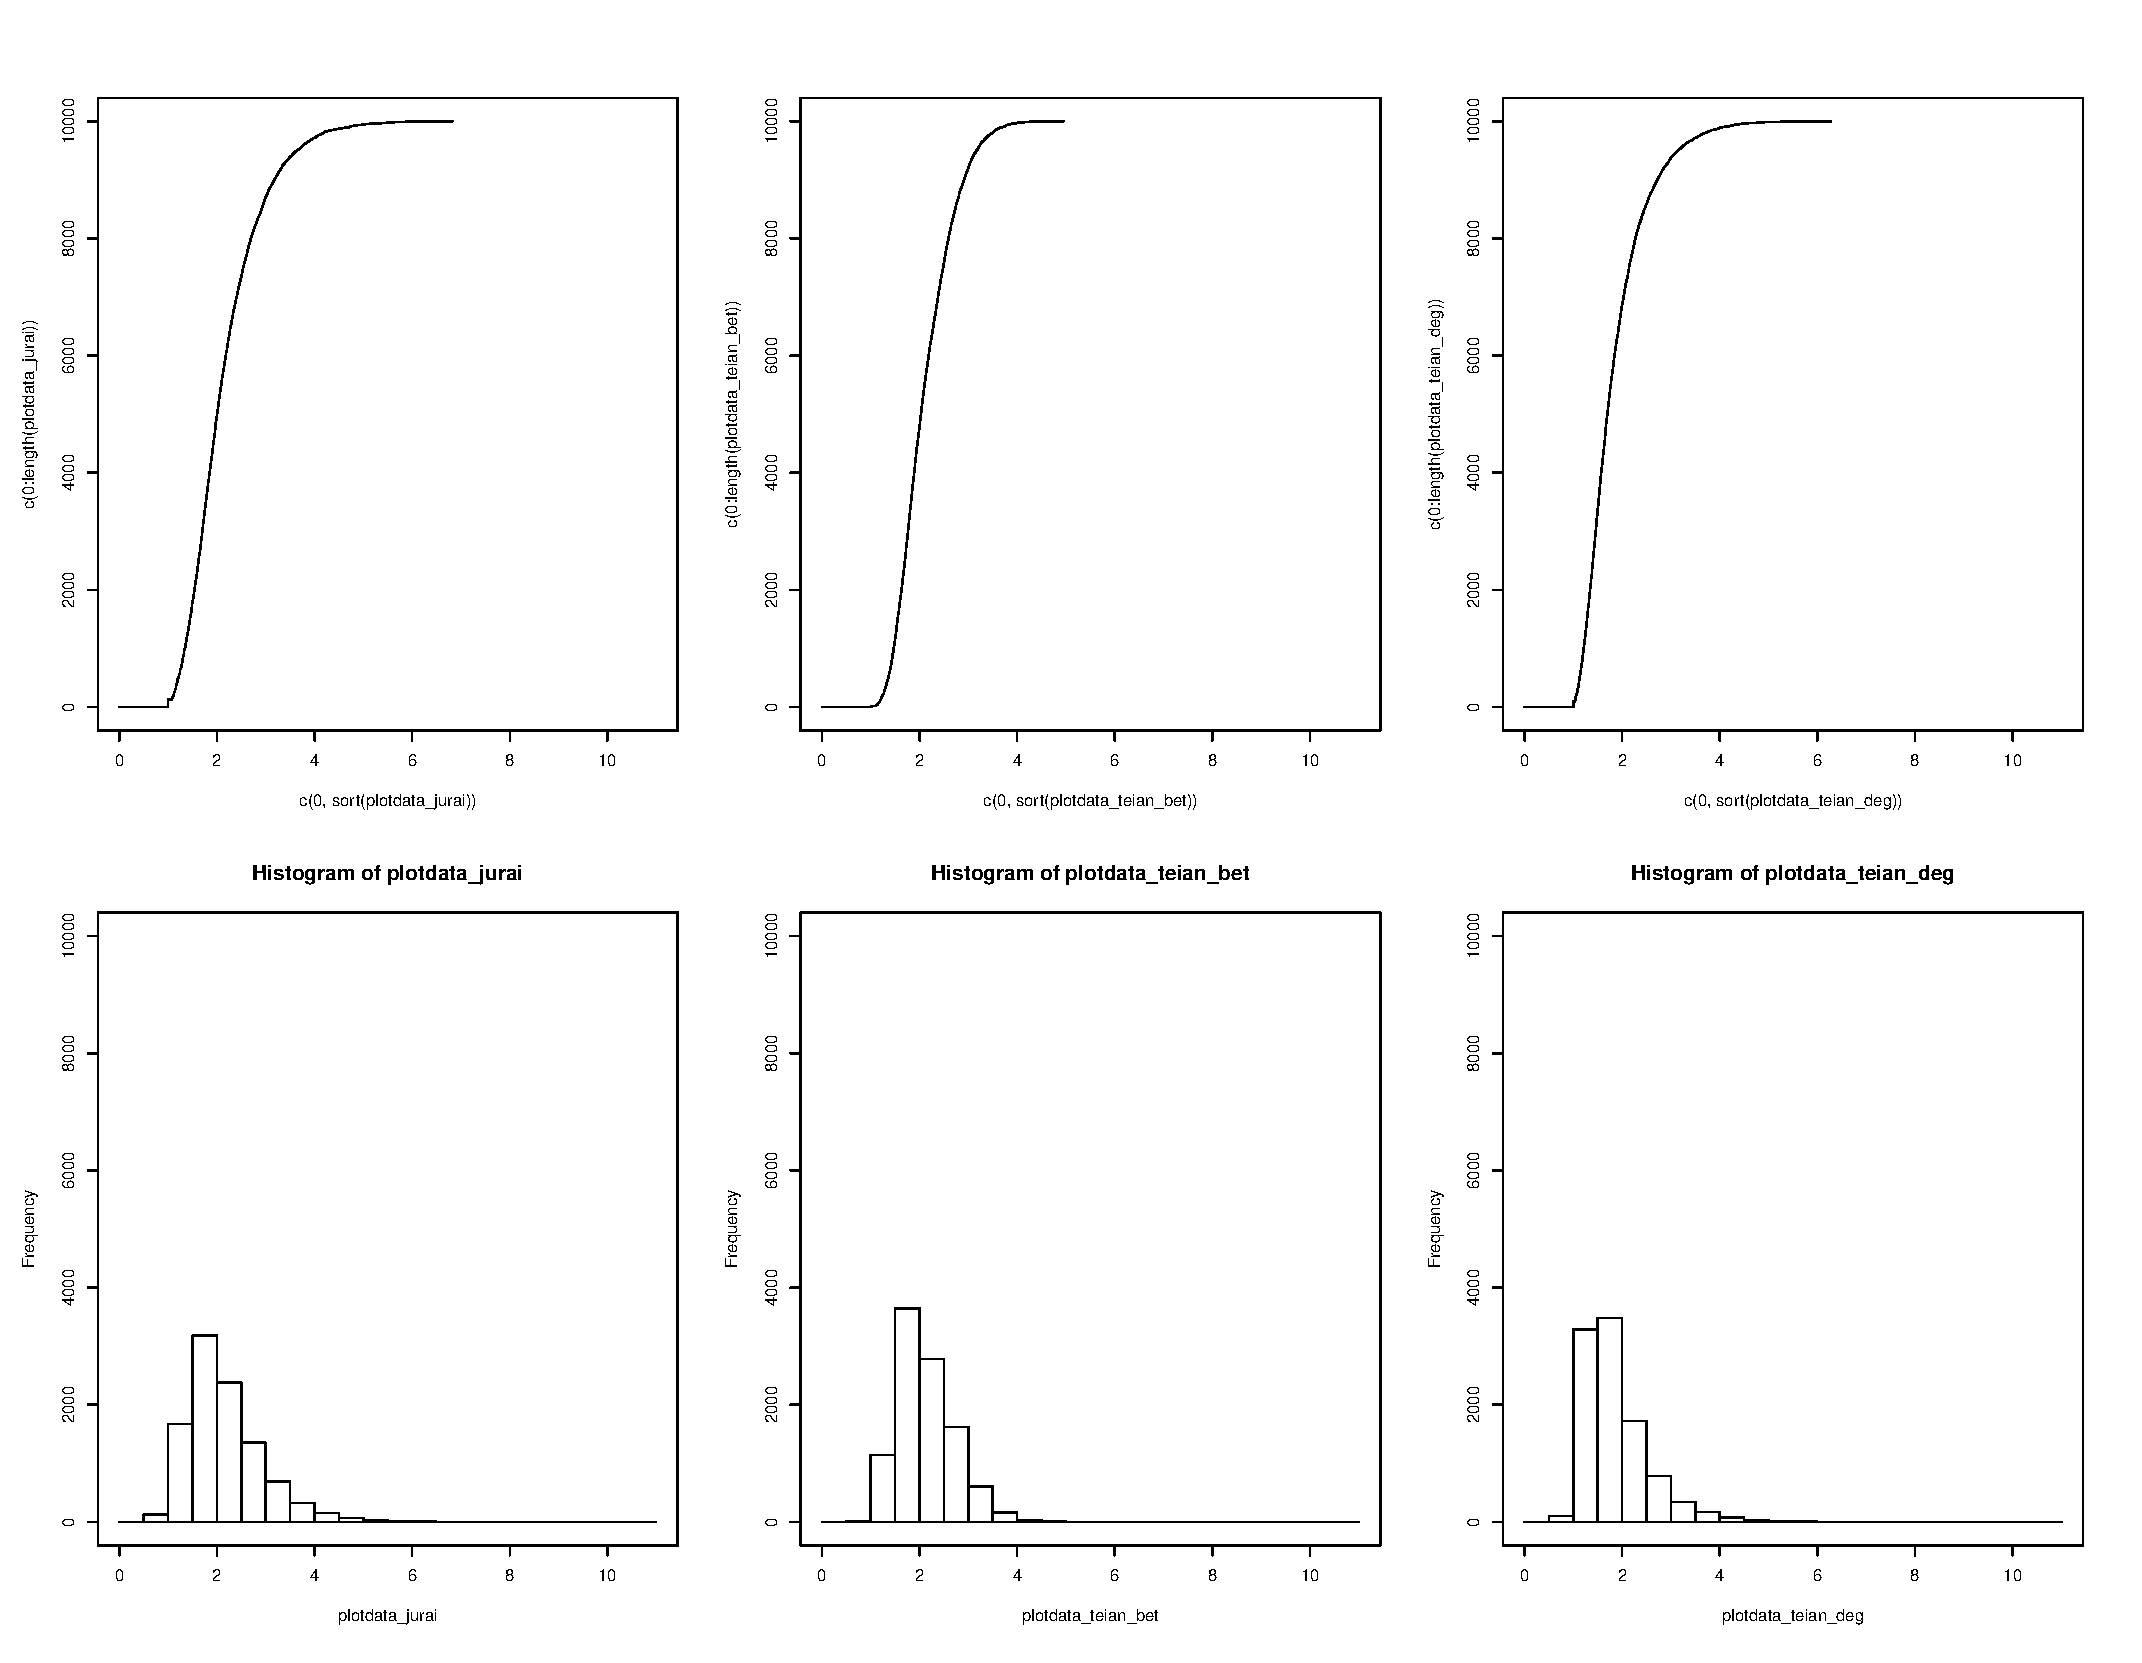
\includegraphics[width=1.2\textwidth]{figures/1_50_30.eps}
  \caption{方法1:50ノードで到達範囲を30としたとき}
  \label{fig:1_50_30}
\end{figure}

\begin{figure}[H]
  \centering
  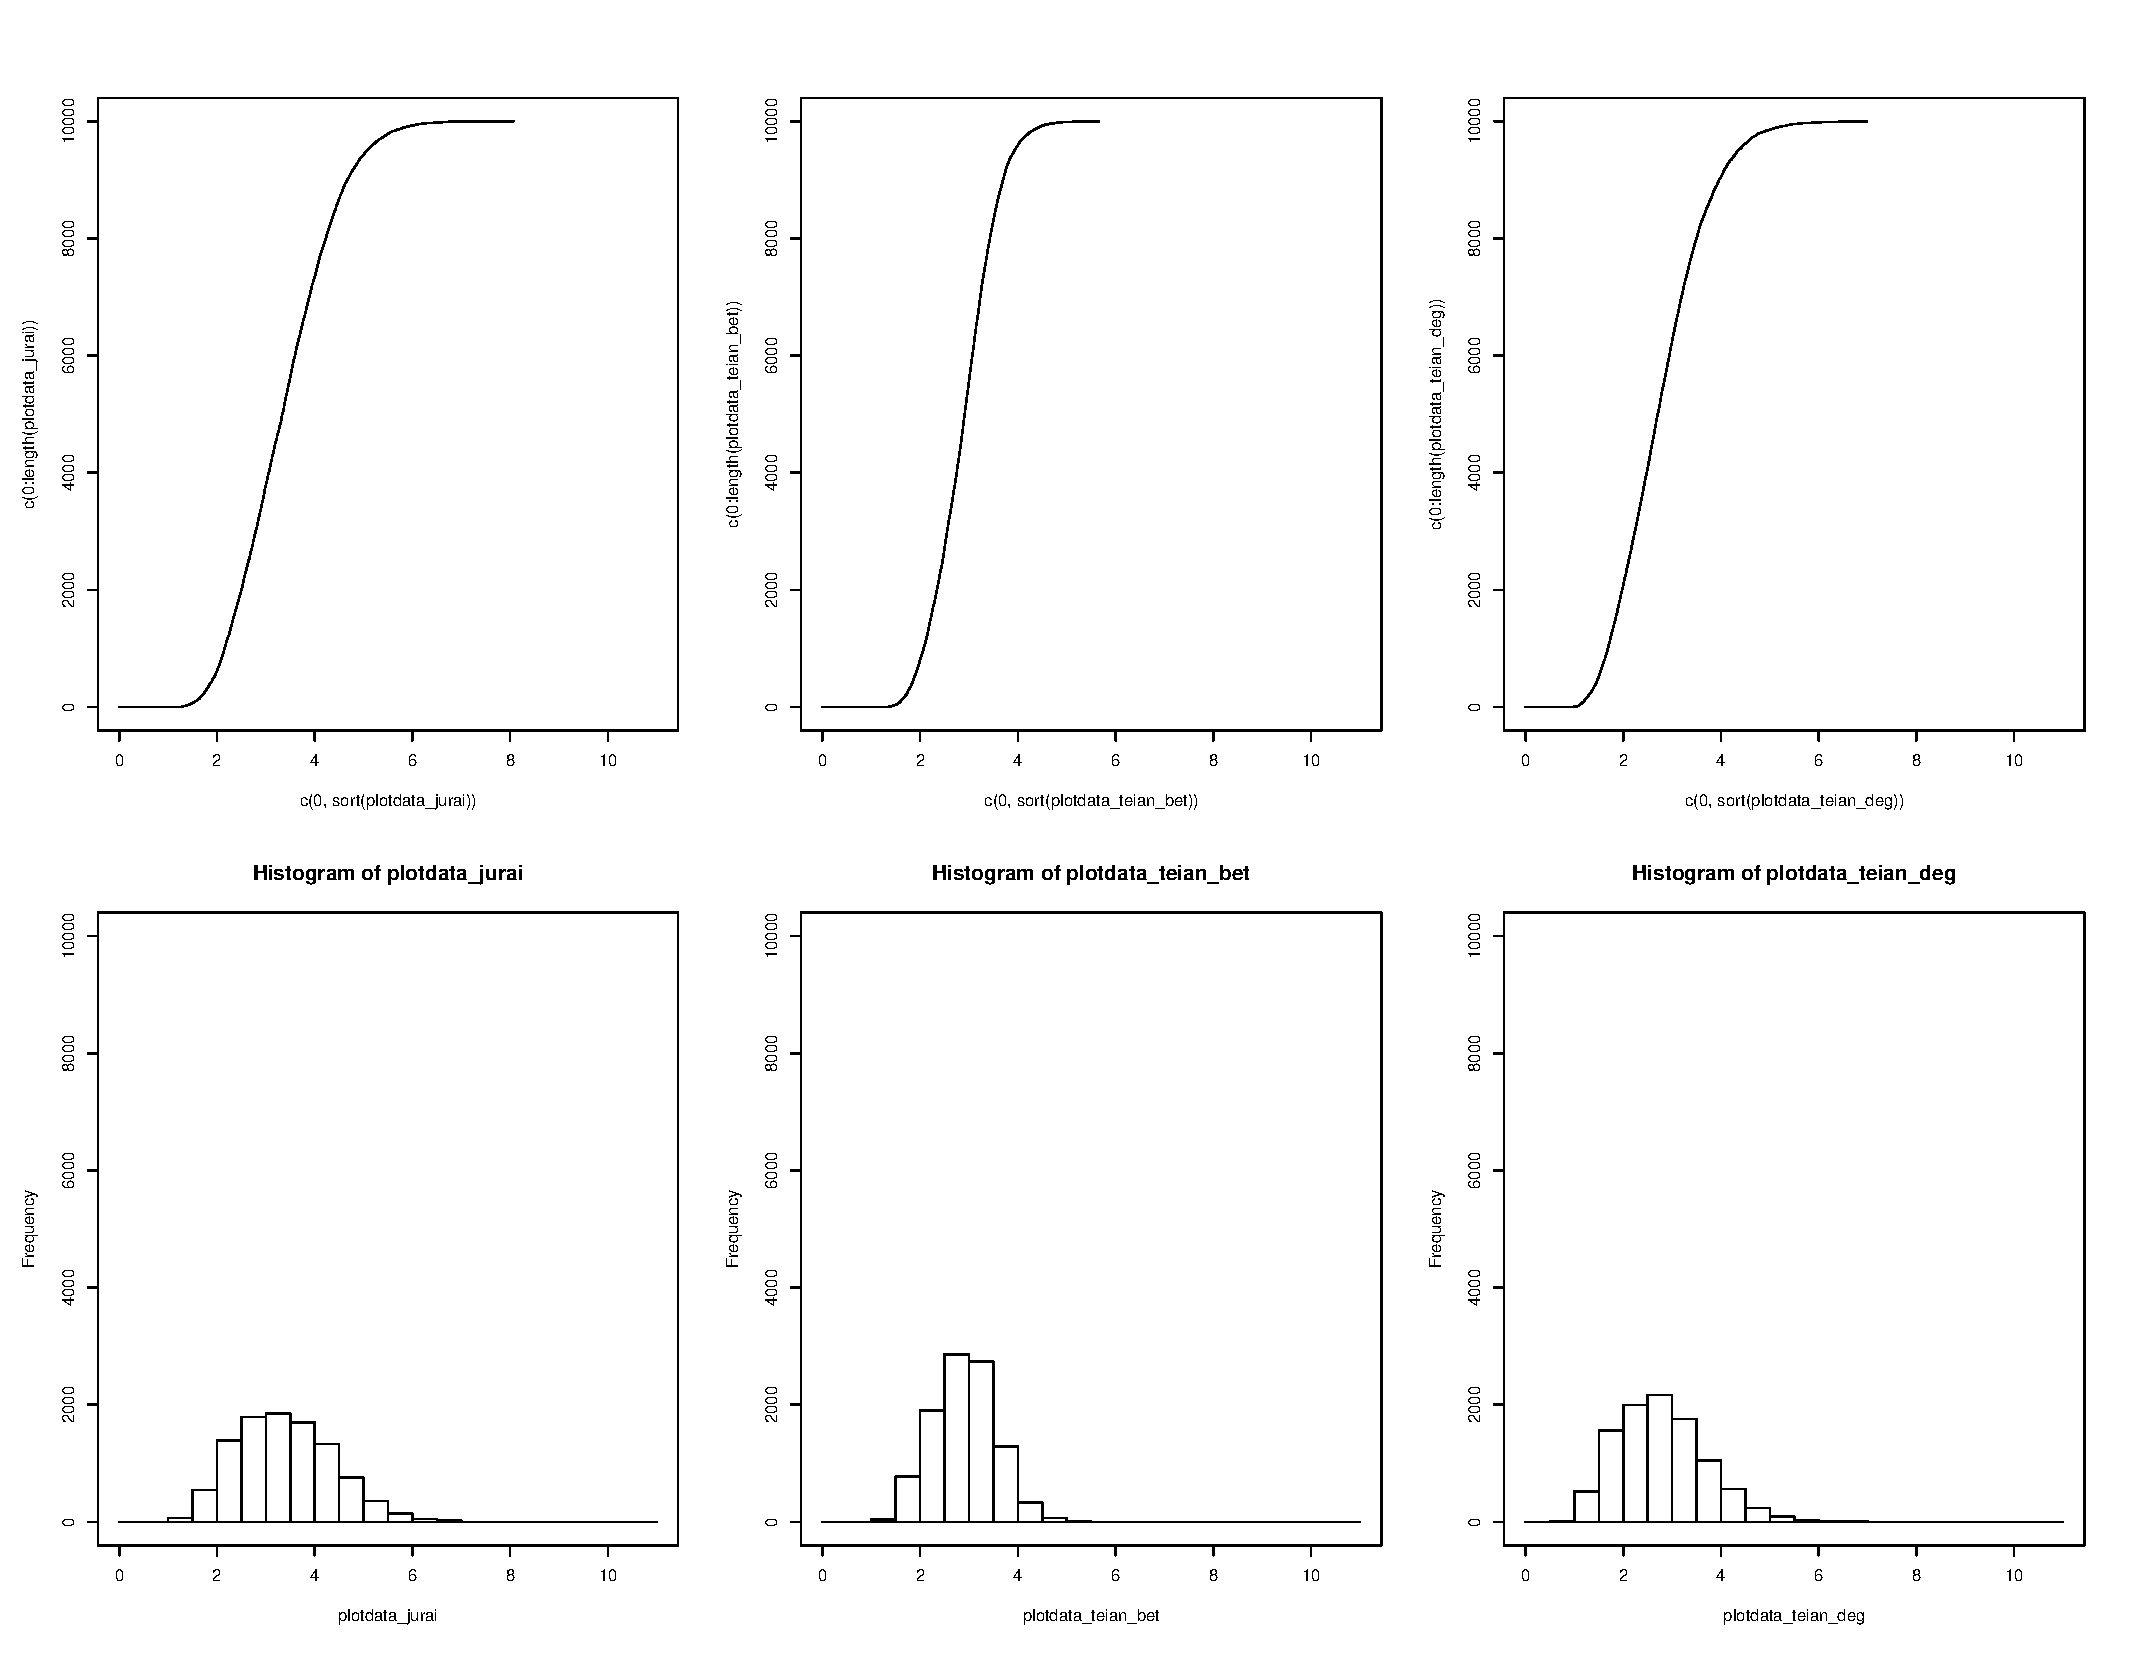
\includegraphics[width=1.2\textwidth]{figures/1_50_40.eps}
  \caption{方法1:50ノードで到達範囲を40としたとき}
  \label{fig:plot}
\end{figure}

\begin{figure}[H]
  \centering
  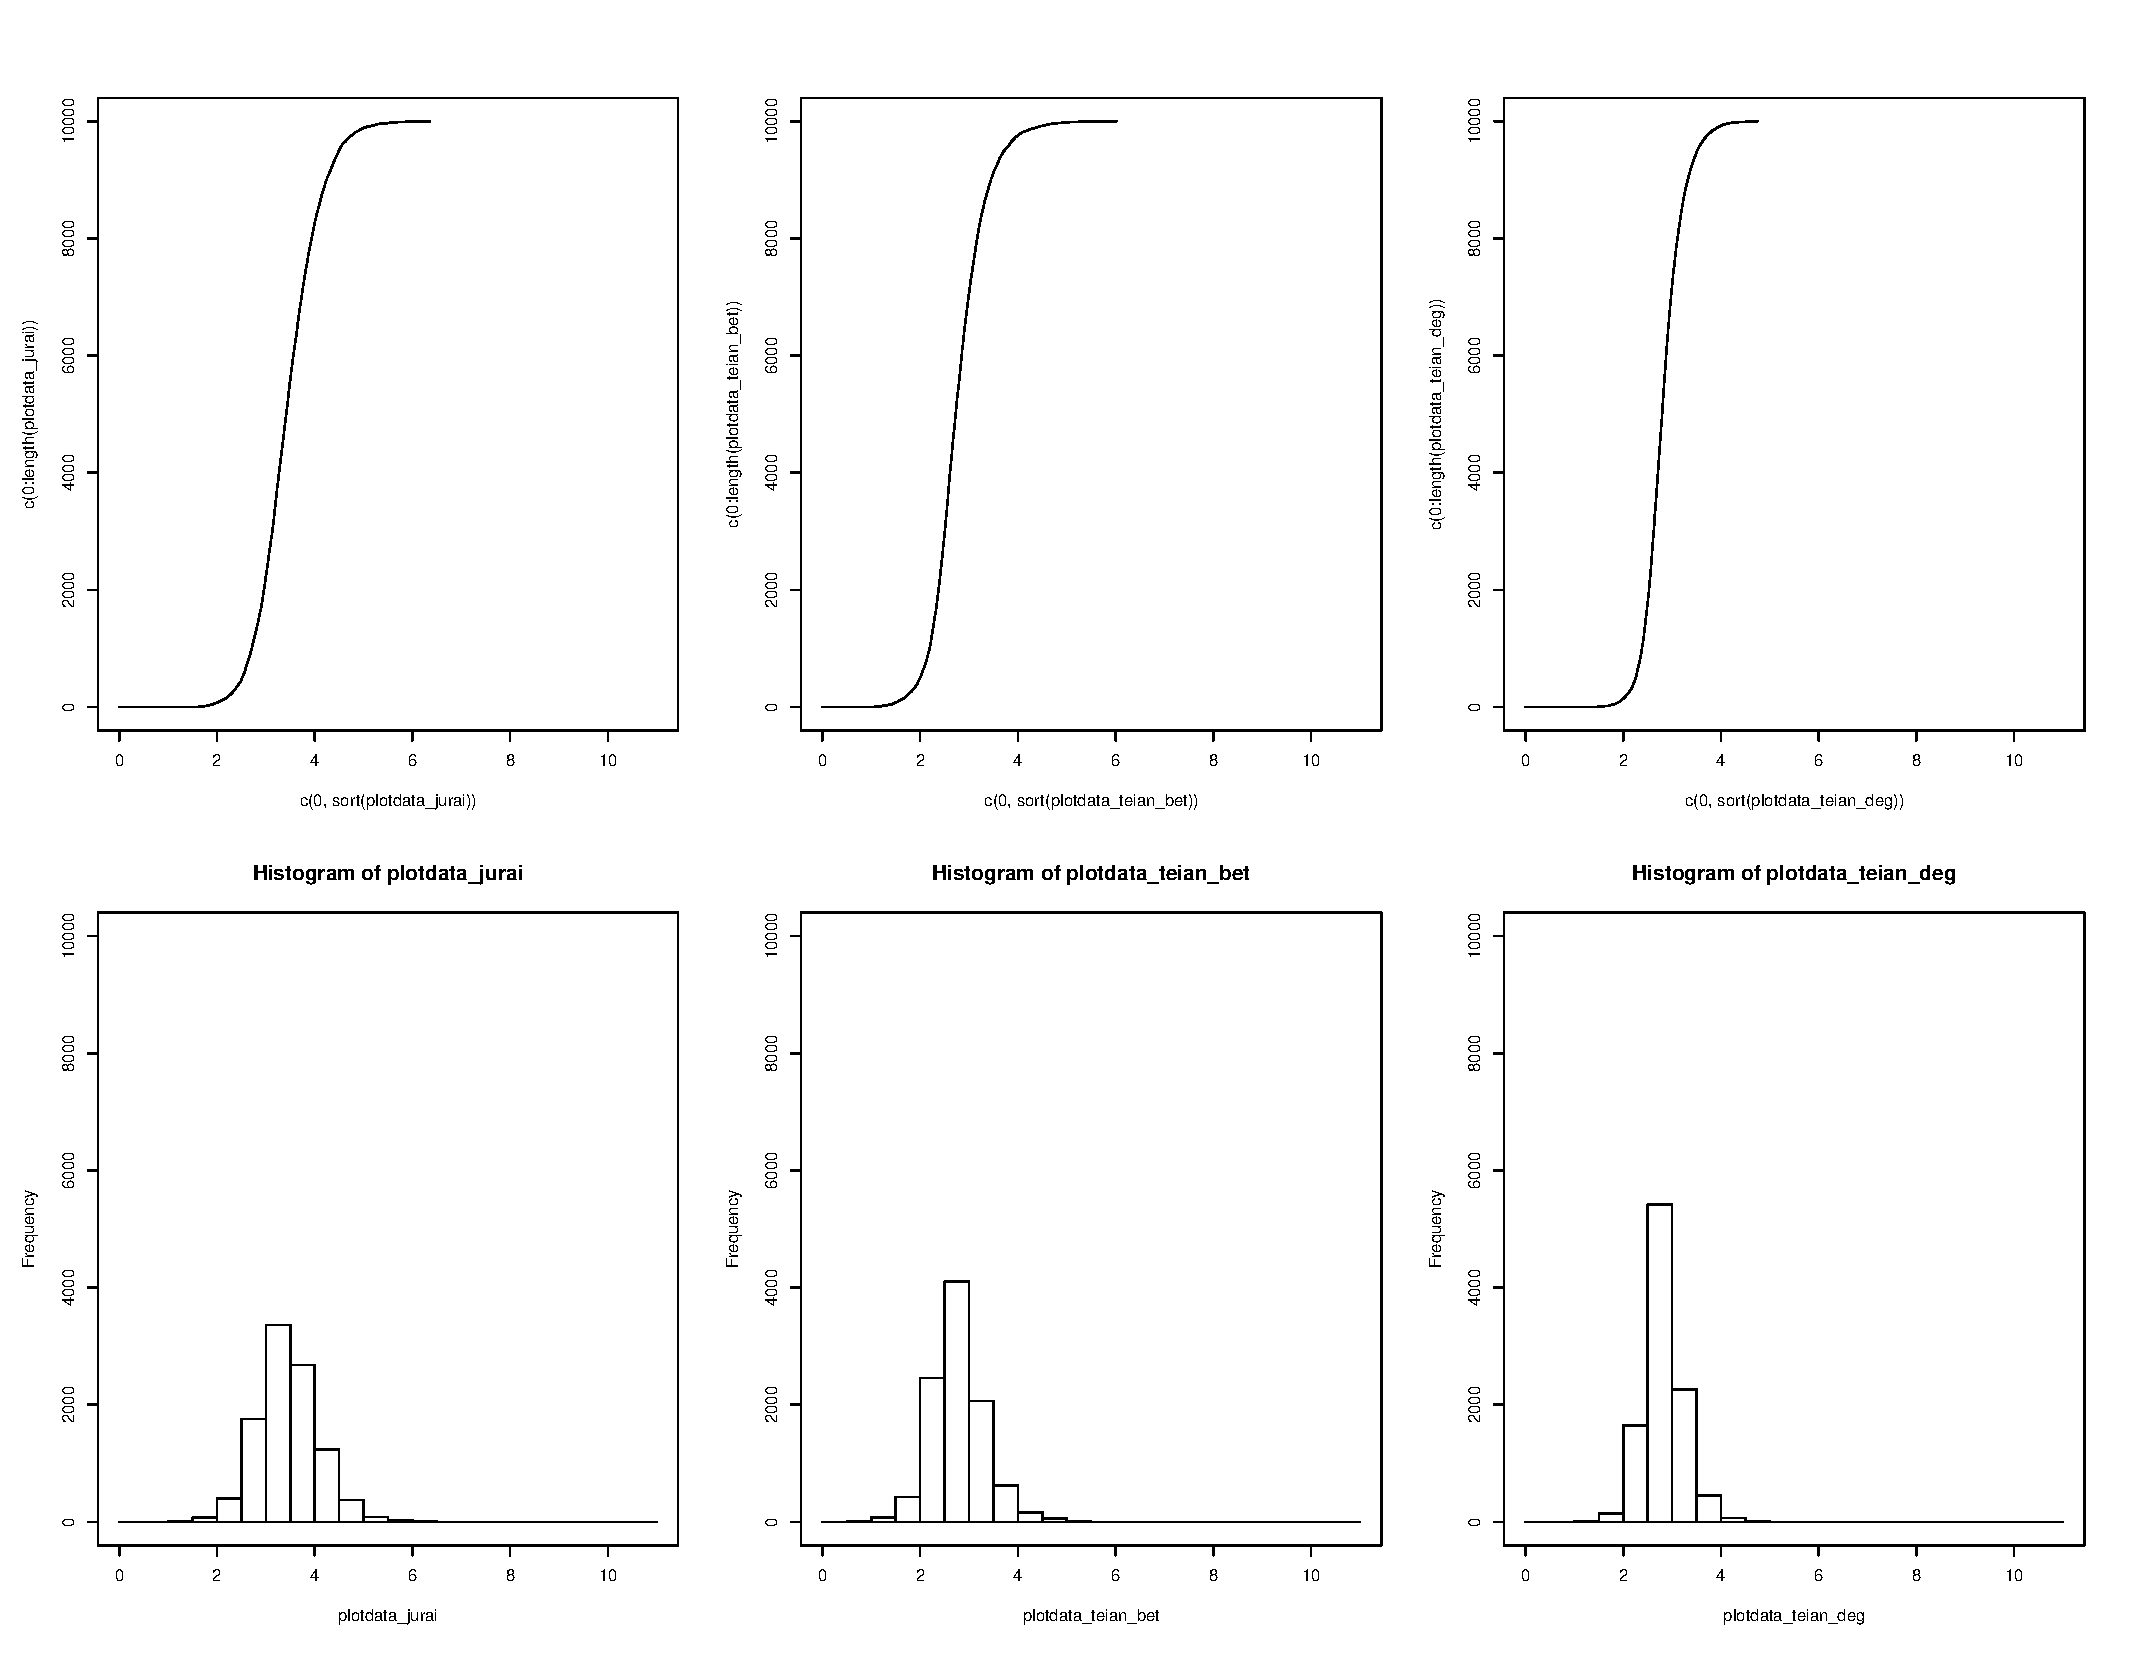
\includegraphics[width=1.2\textwidth]{figures/1_50_50.eps}
  \caption{方法1:50ノードで到達範囲を50としたとき}
  \label{fig:plot}
\end{figure}

\begin{figure}[H]
  \centering
  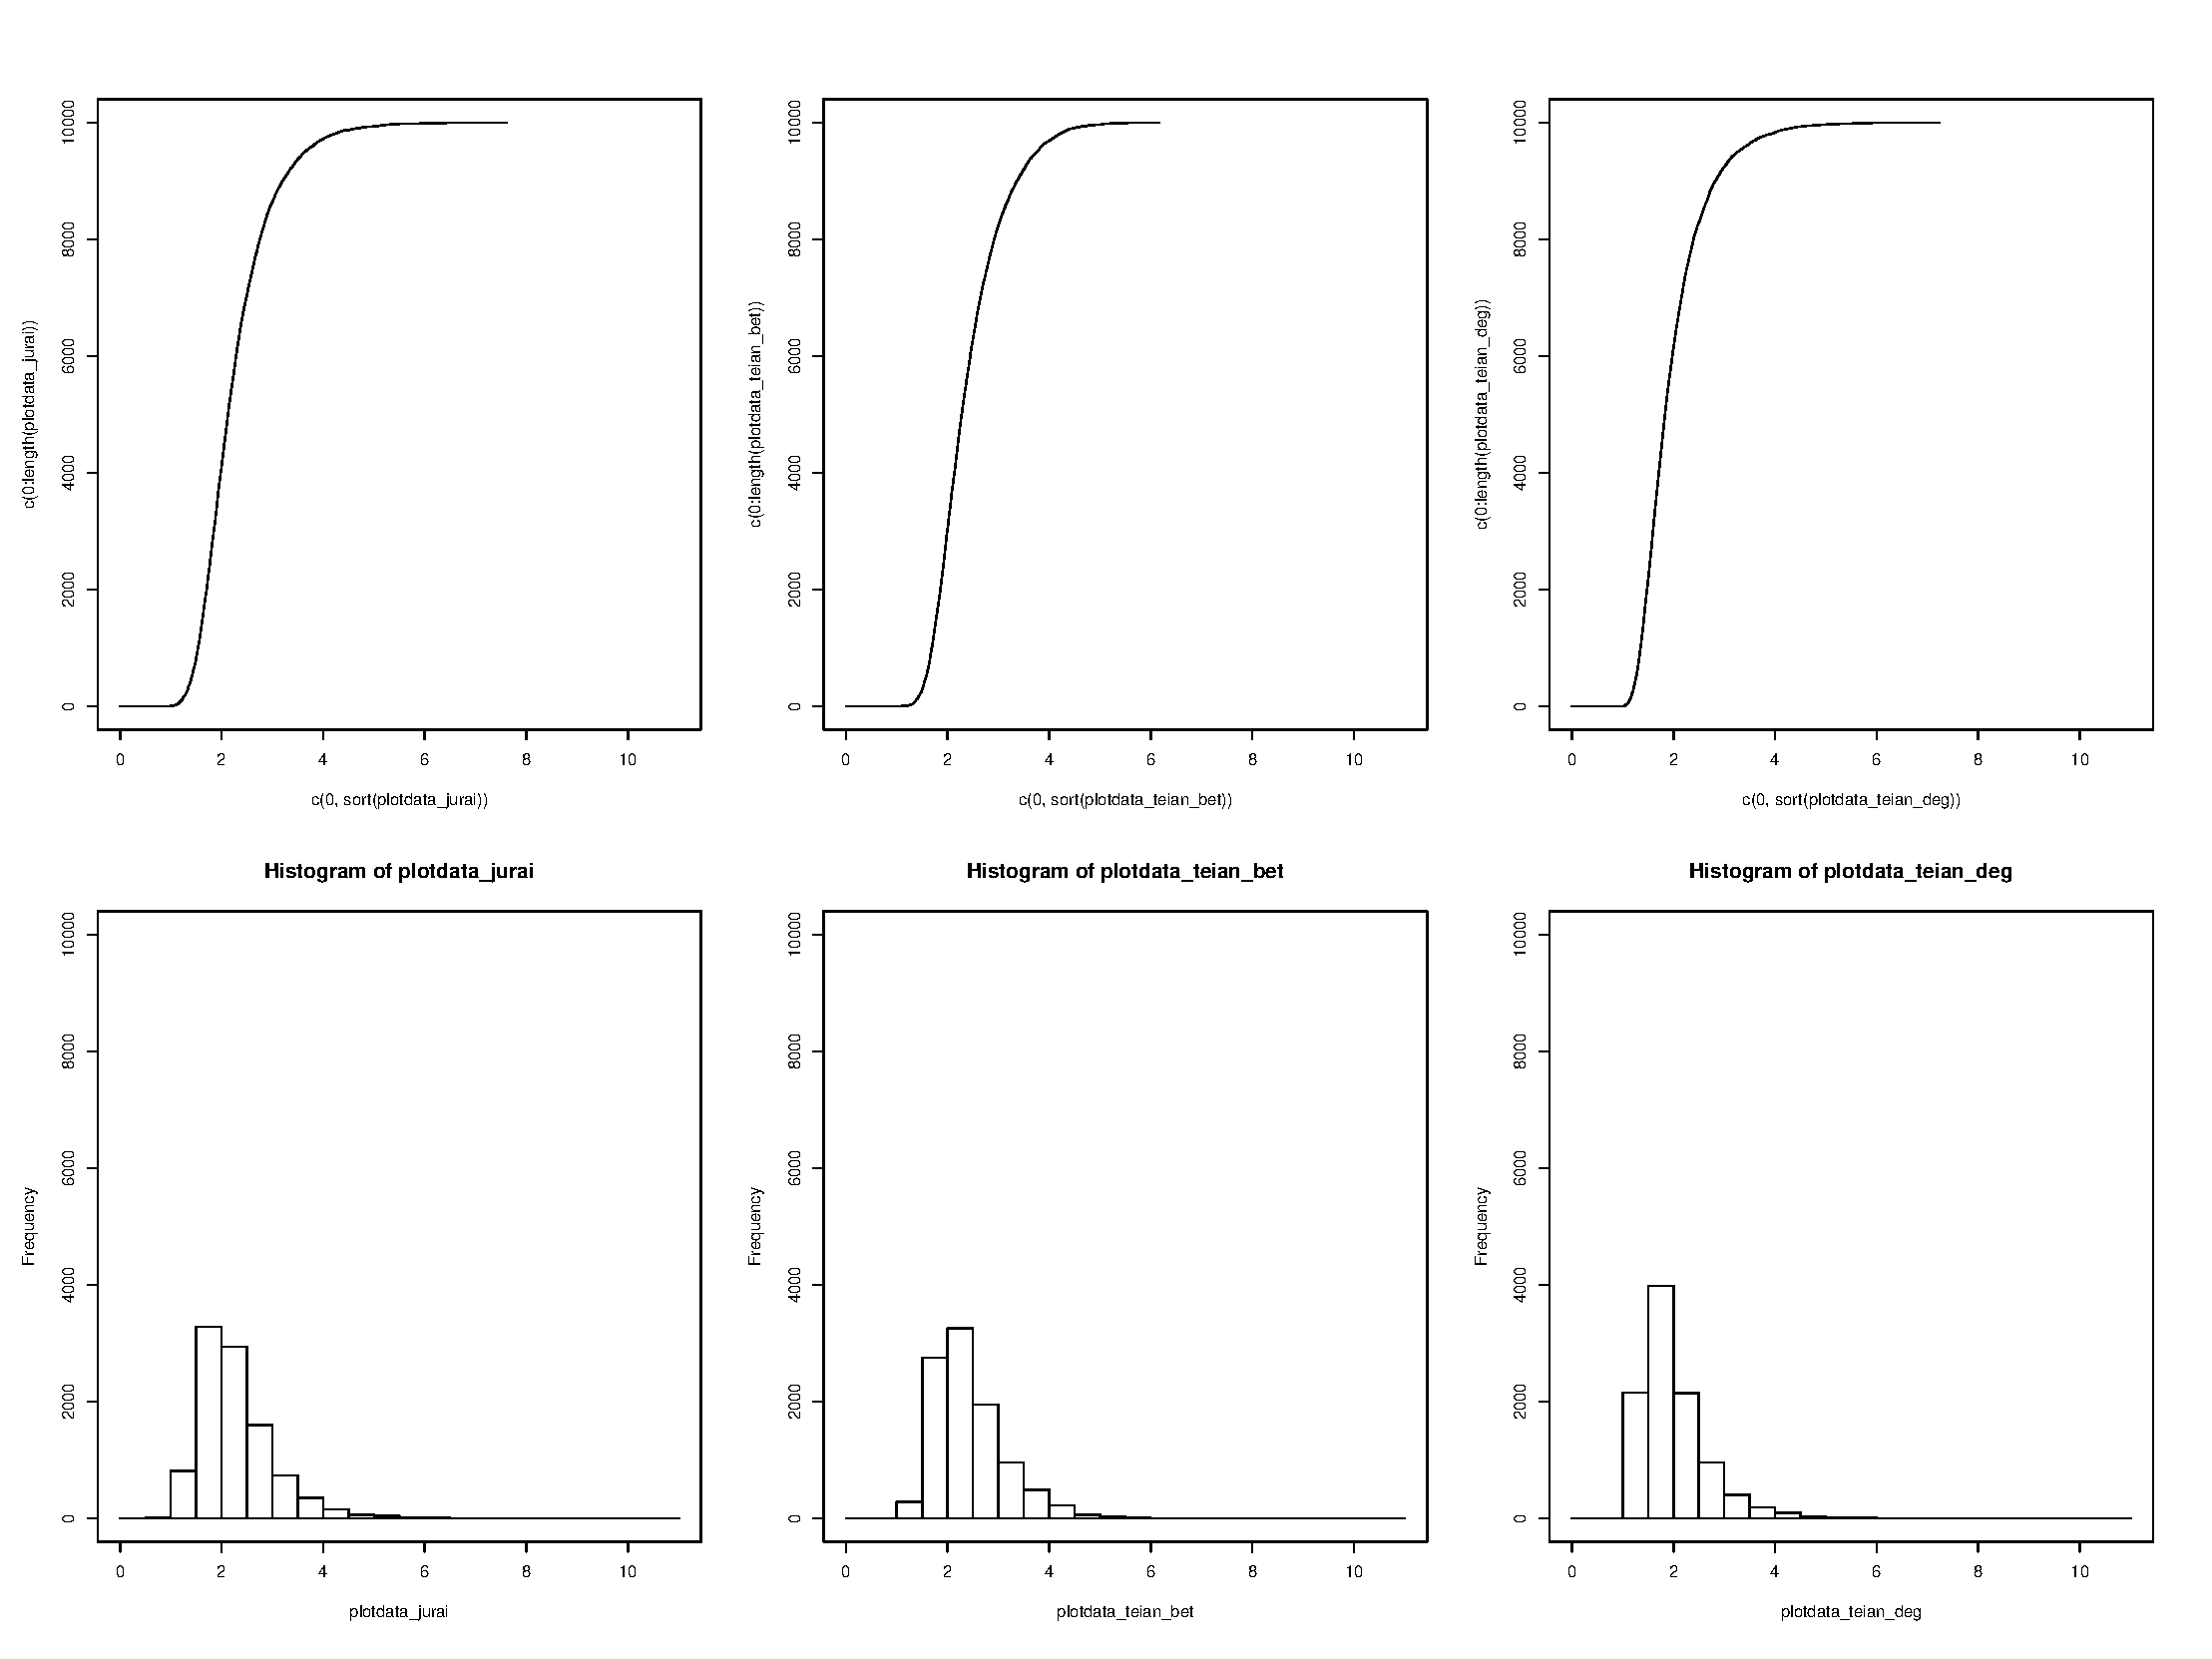
\includegraphics[width=1.2\textwidth]{figures/1_100_20.eps}
  \caption{方法1:100ノードで到達範囲を20としたとき}
  \label{fig:plot}
\end{figure}


\begin{figure}[H]
  \centering
  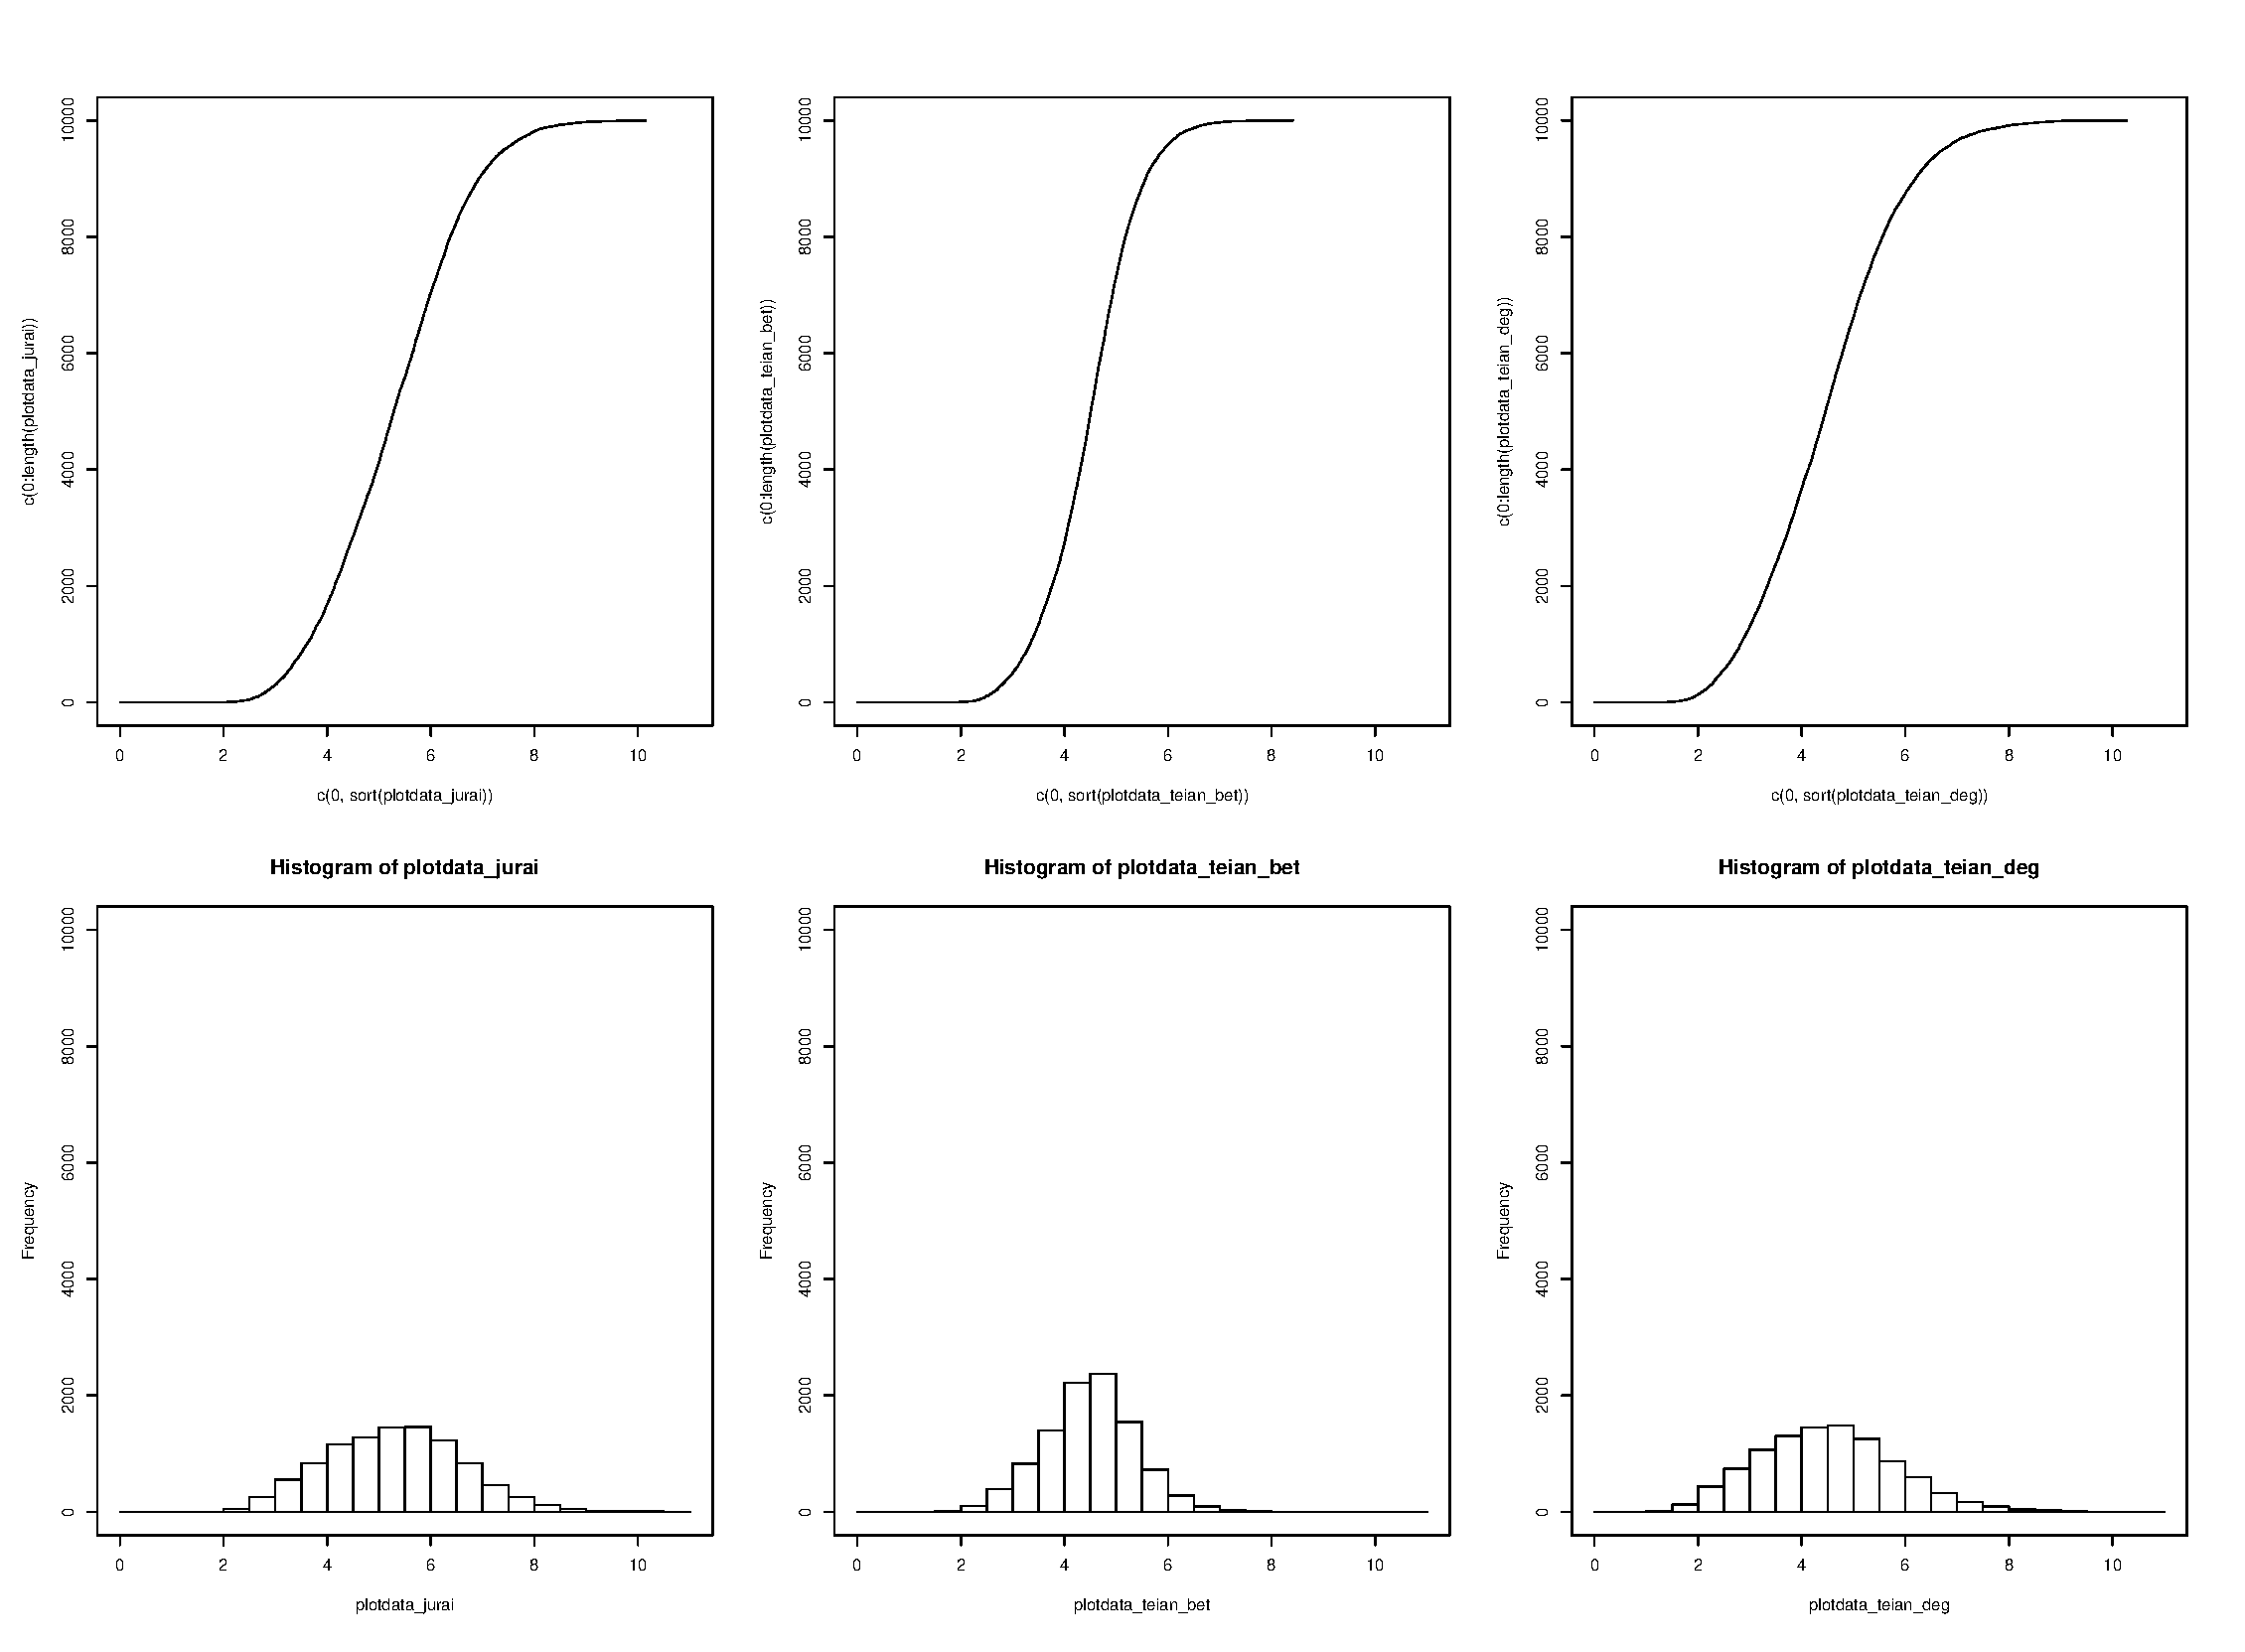
\includegraphics[width=1.2\textwidth]{figures/1_100_30.eps}
  \caption{方法1:100ノードで到達範囲を30としたとき}
  \label{fig:plot}
\end{figure}

\begin{figure}[H]
  \centering
  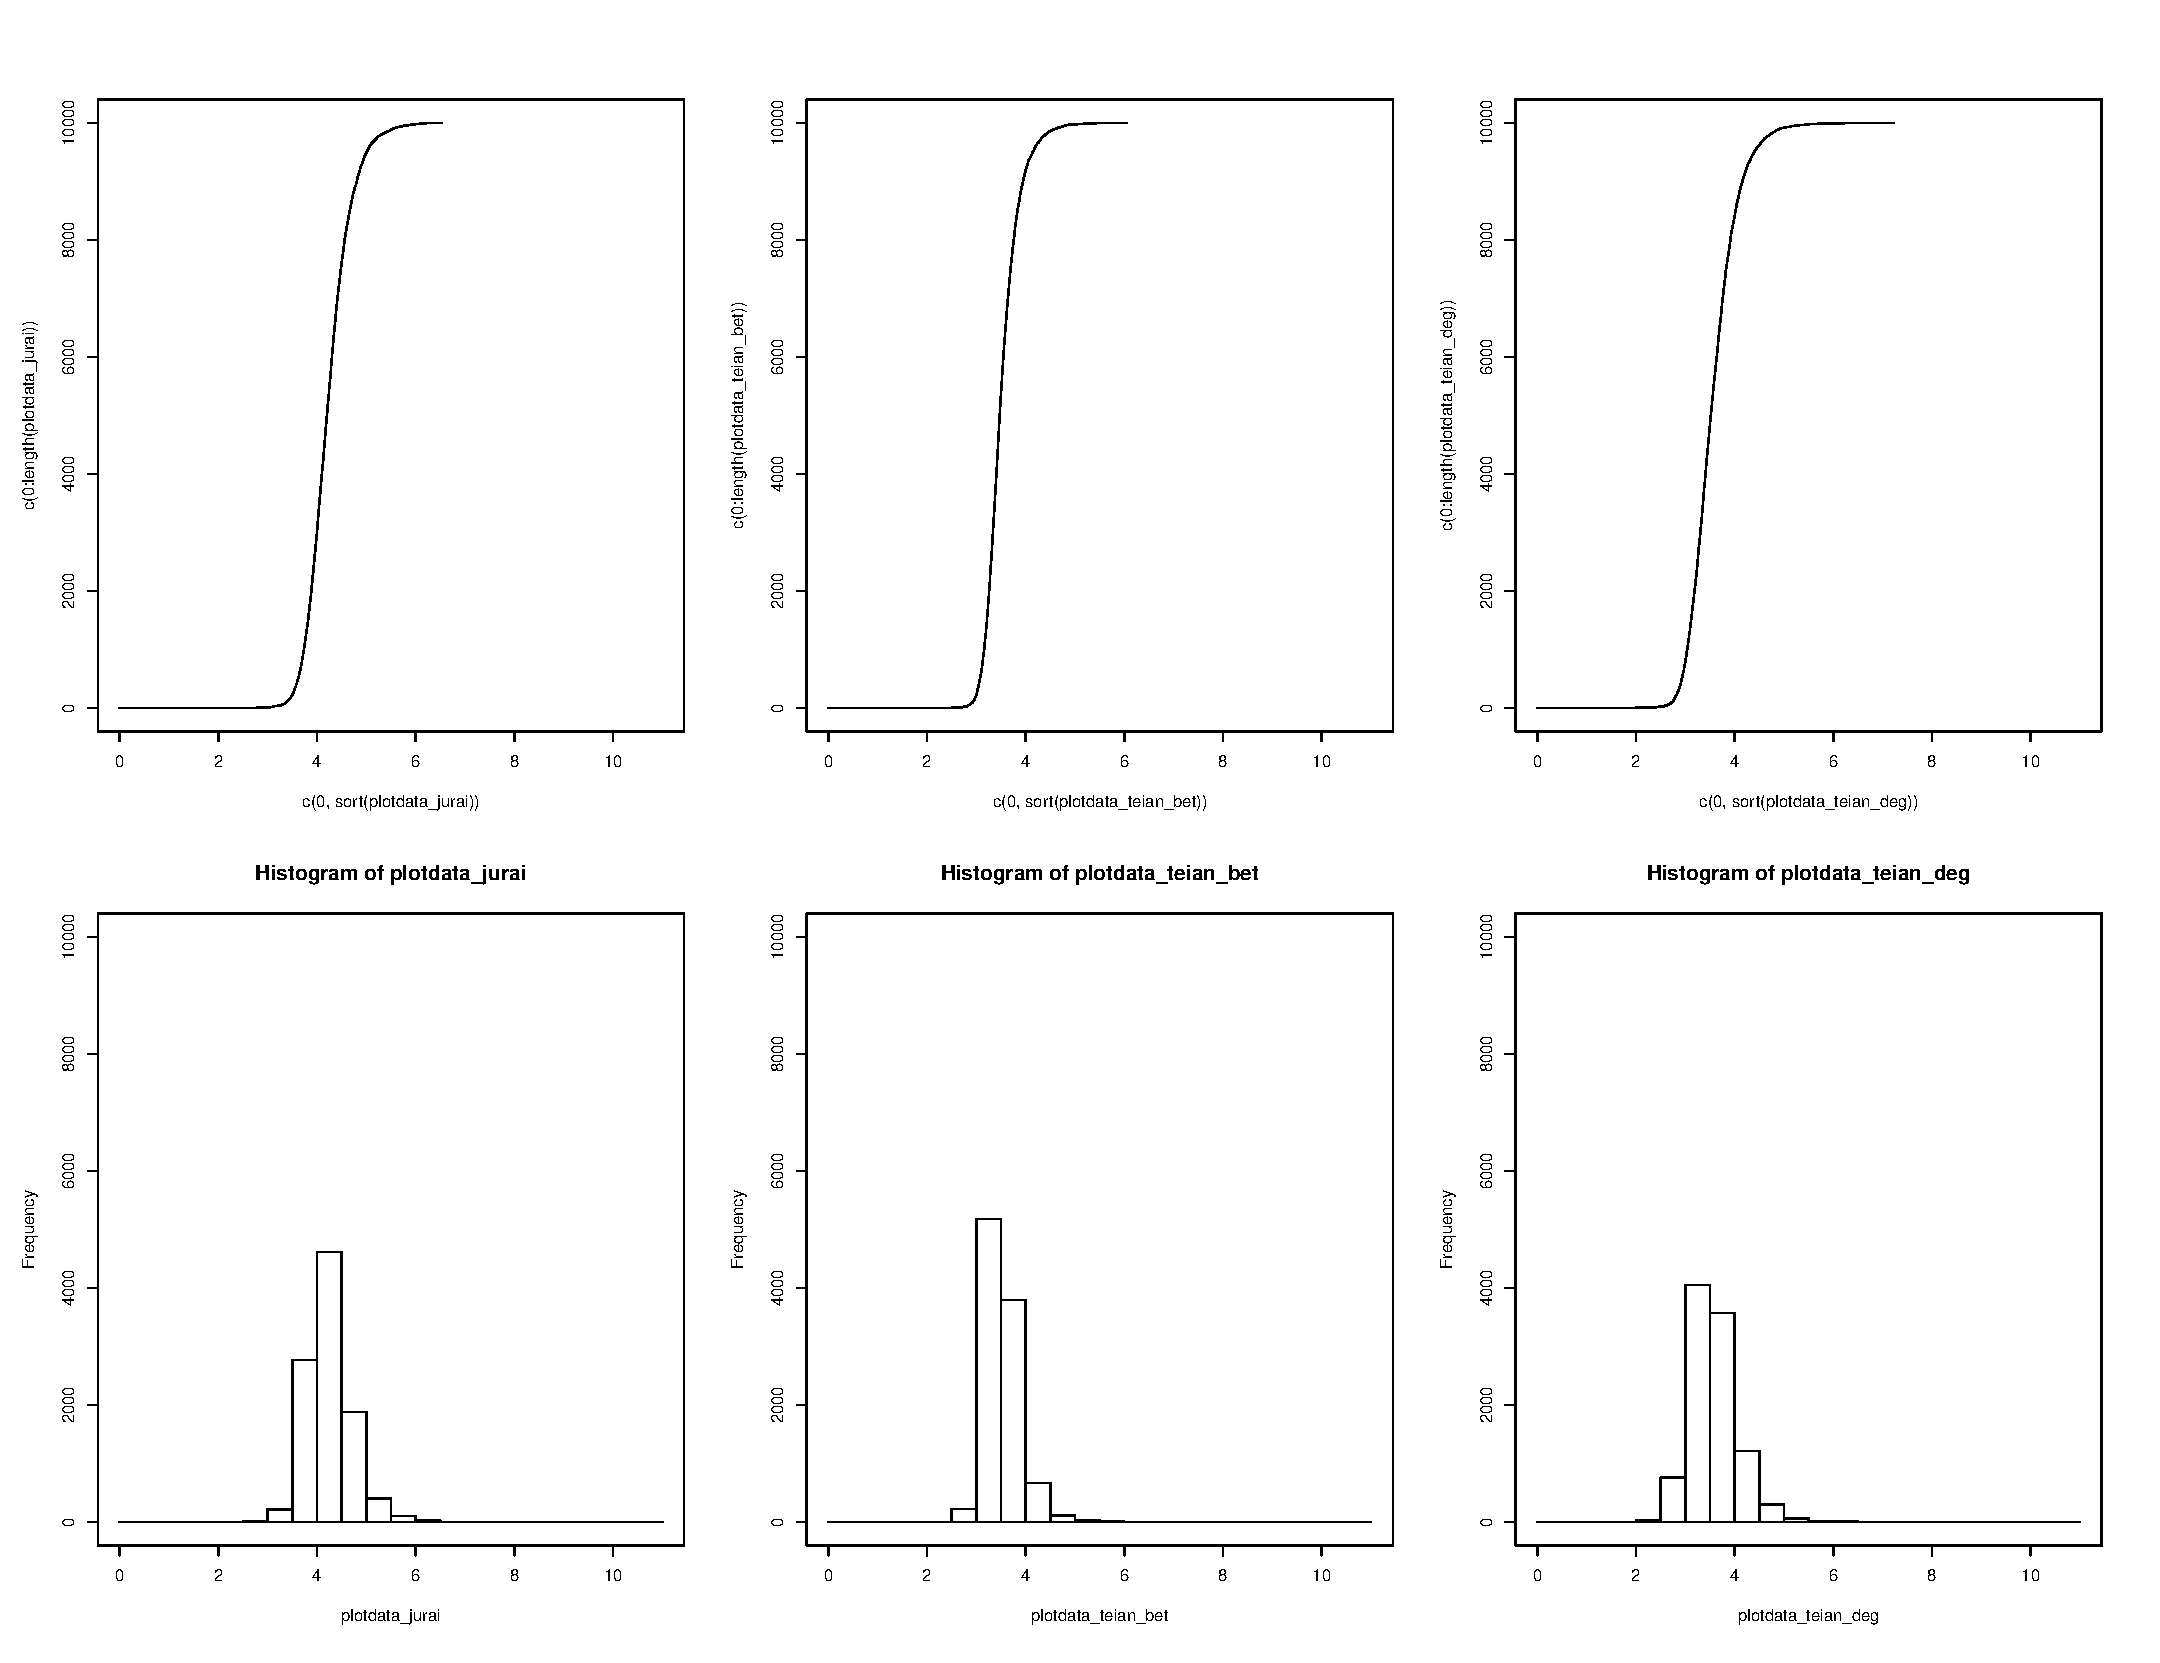
\includegraphics[width=1.2\textwidth]{figures/1_100_40.eps}
  \caption{方法1:100ノードで到達範囲を40としたとき}
  \label{fig:plot}
\end{figure}

\begin{figure}[H]
  \centering
  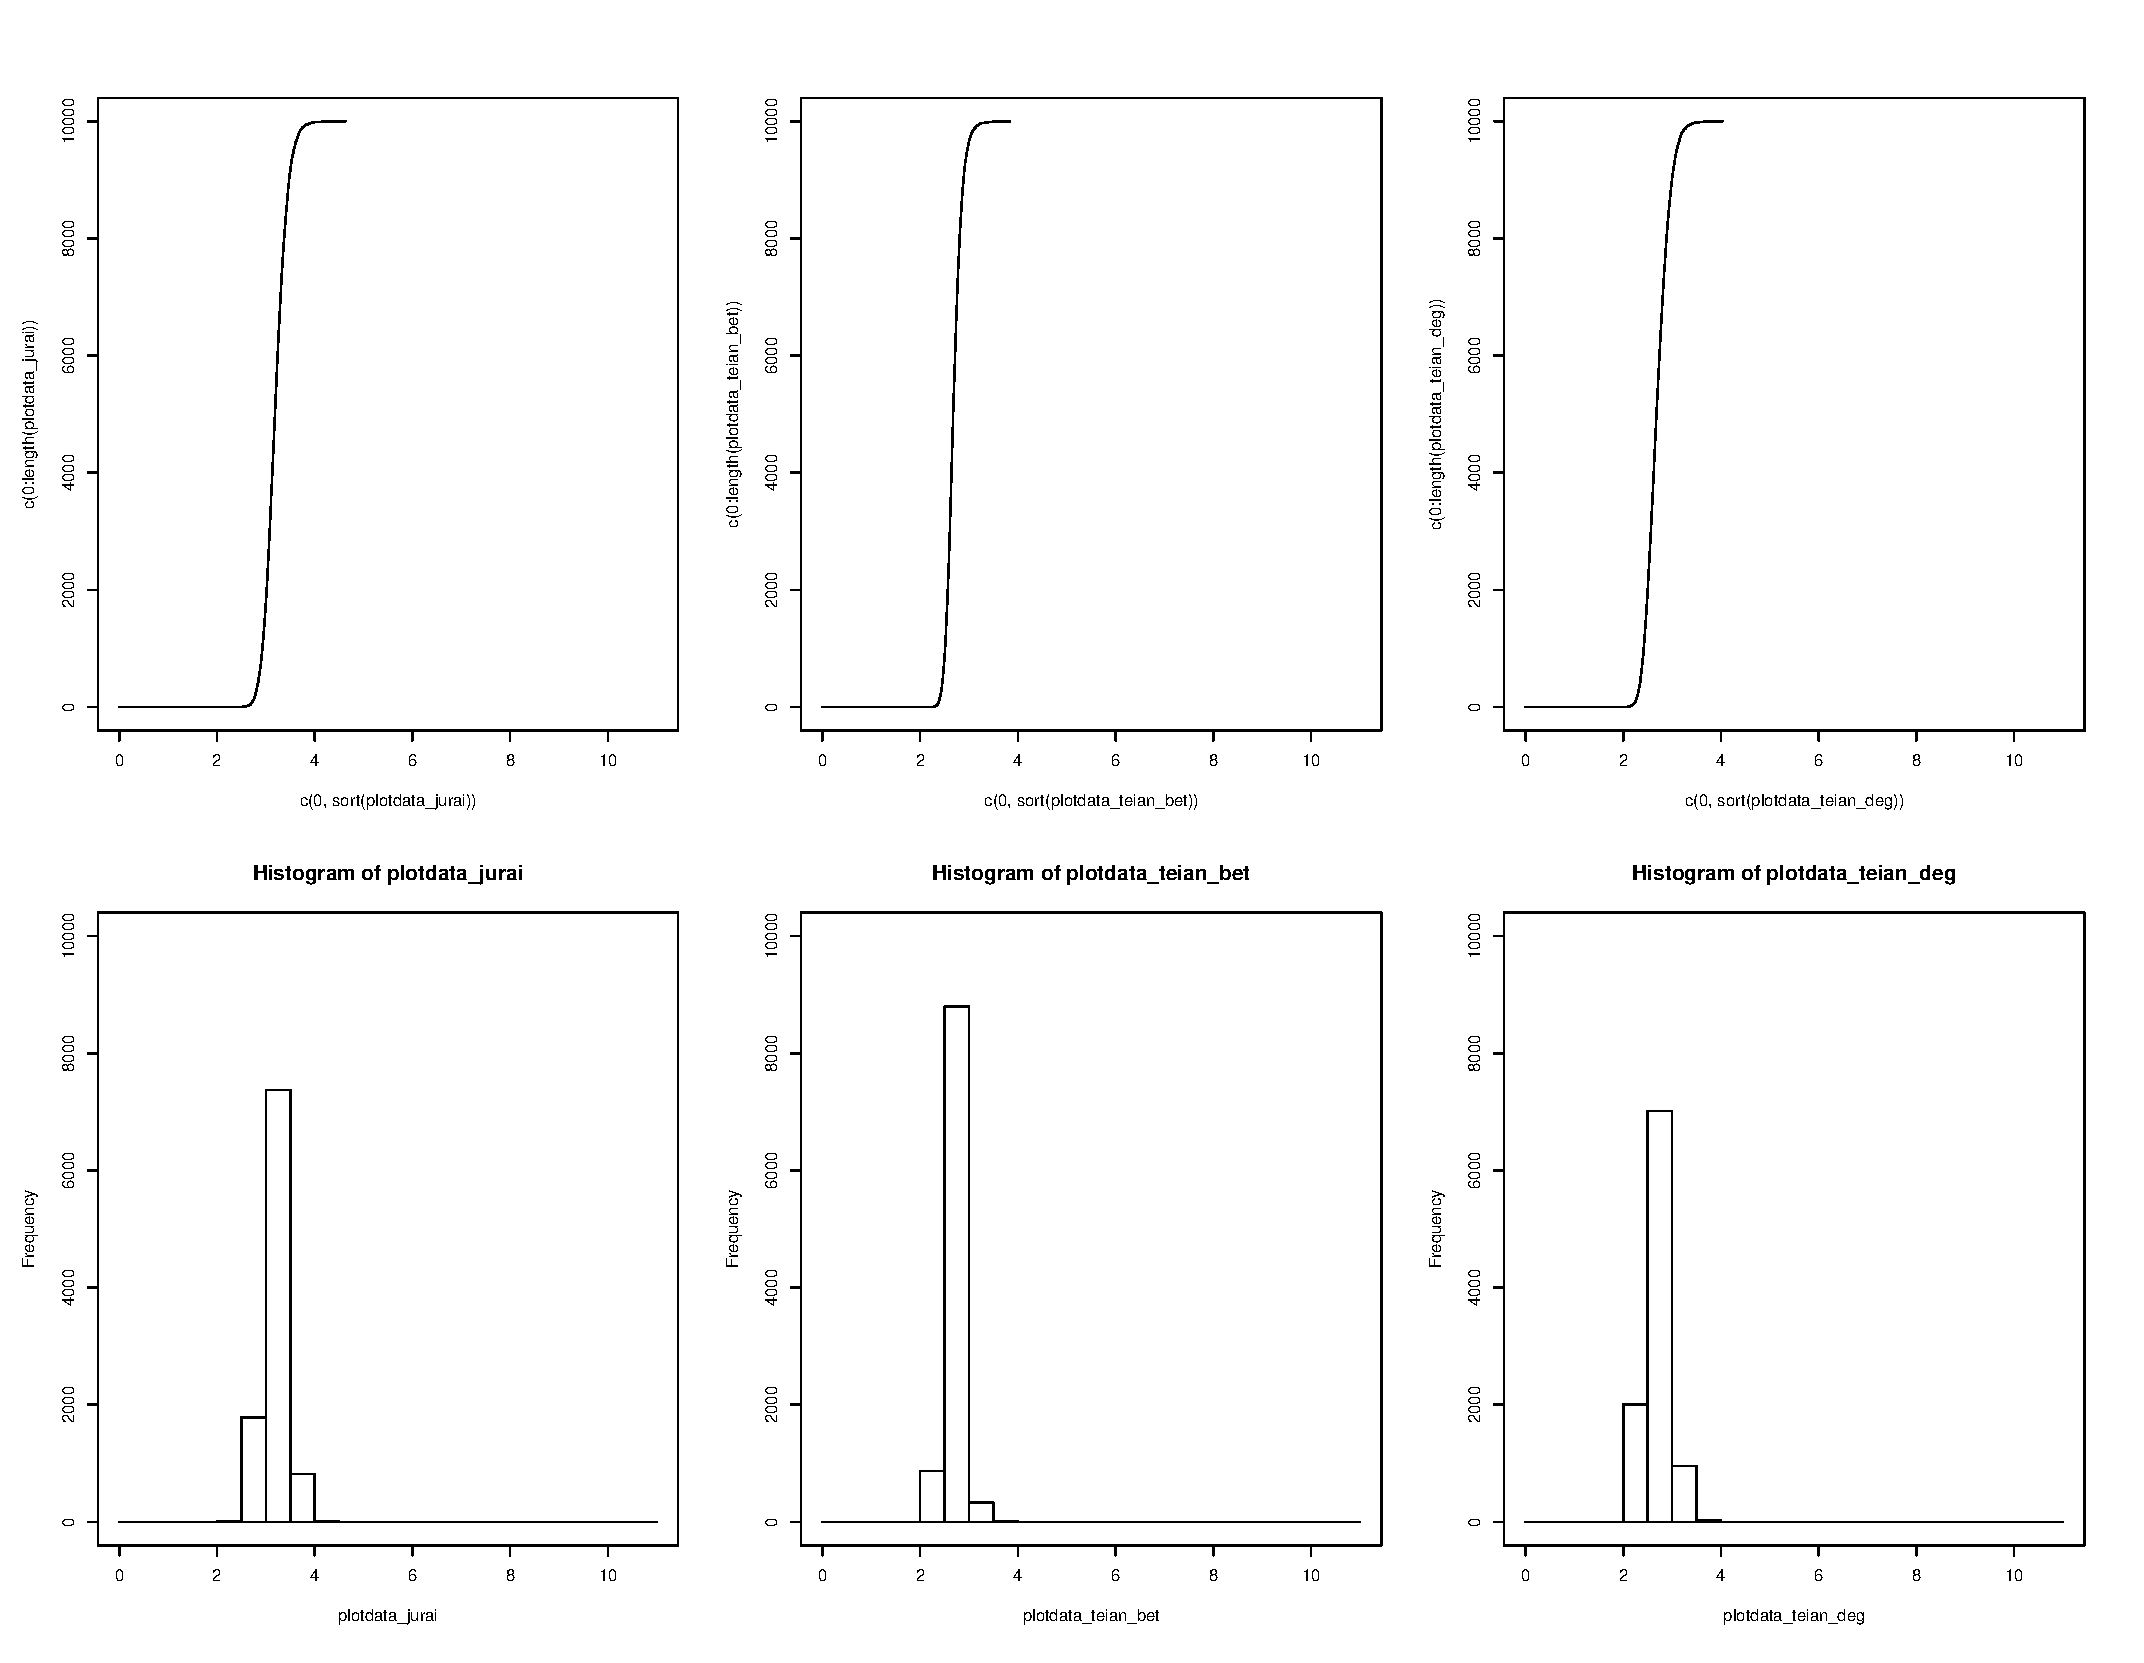
\includegraphics[width=1.2\textwidth]{figures/1_100_50.eps}
  \caption{方法1:100ノードで到達範囲を50としたとき}
  \label{fig:plot}
\end{figure}

\begin{figure}[H]
  \centering
  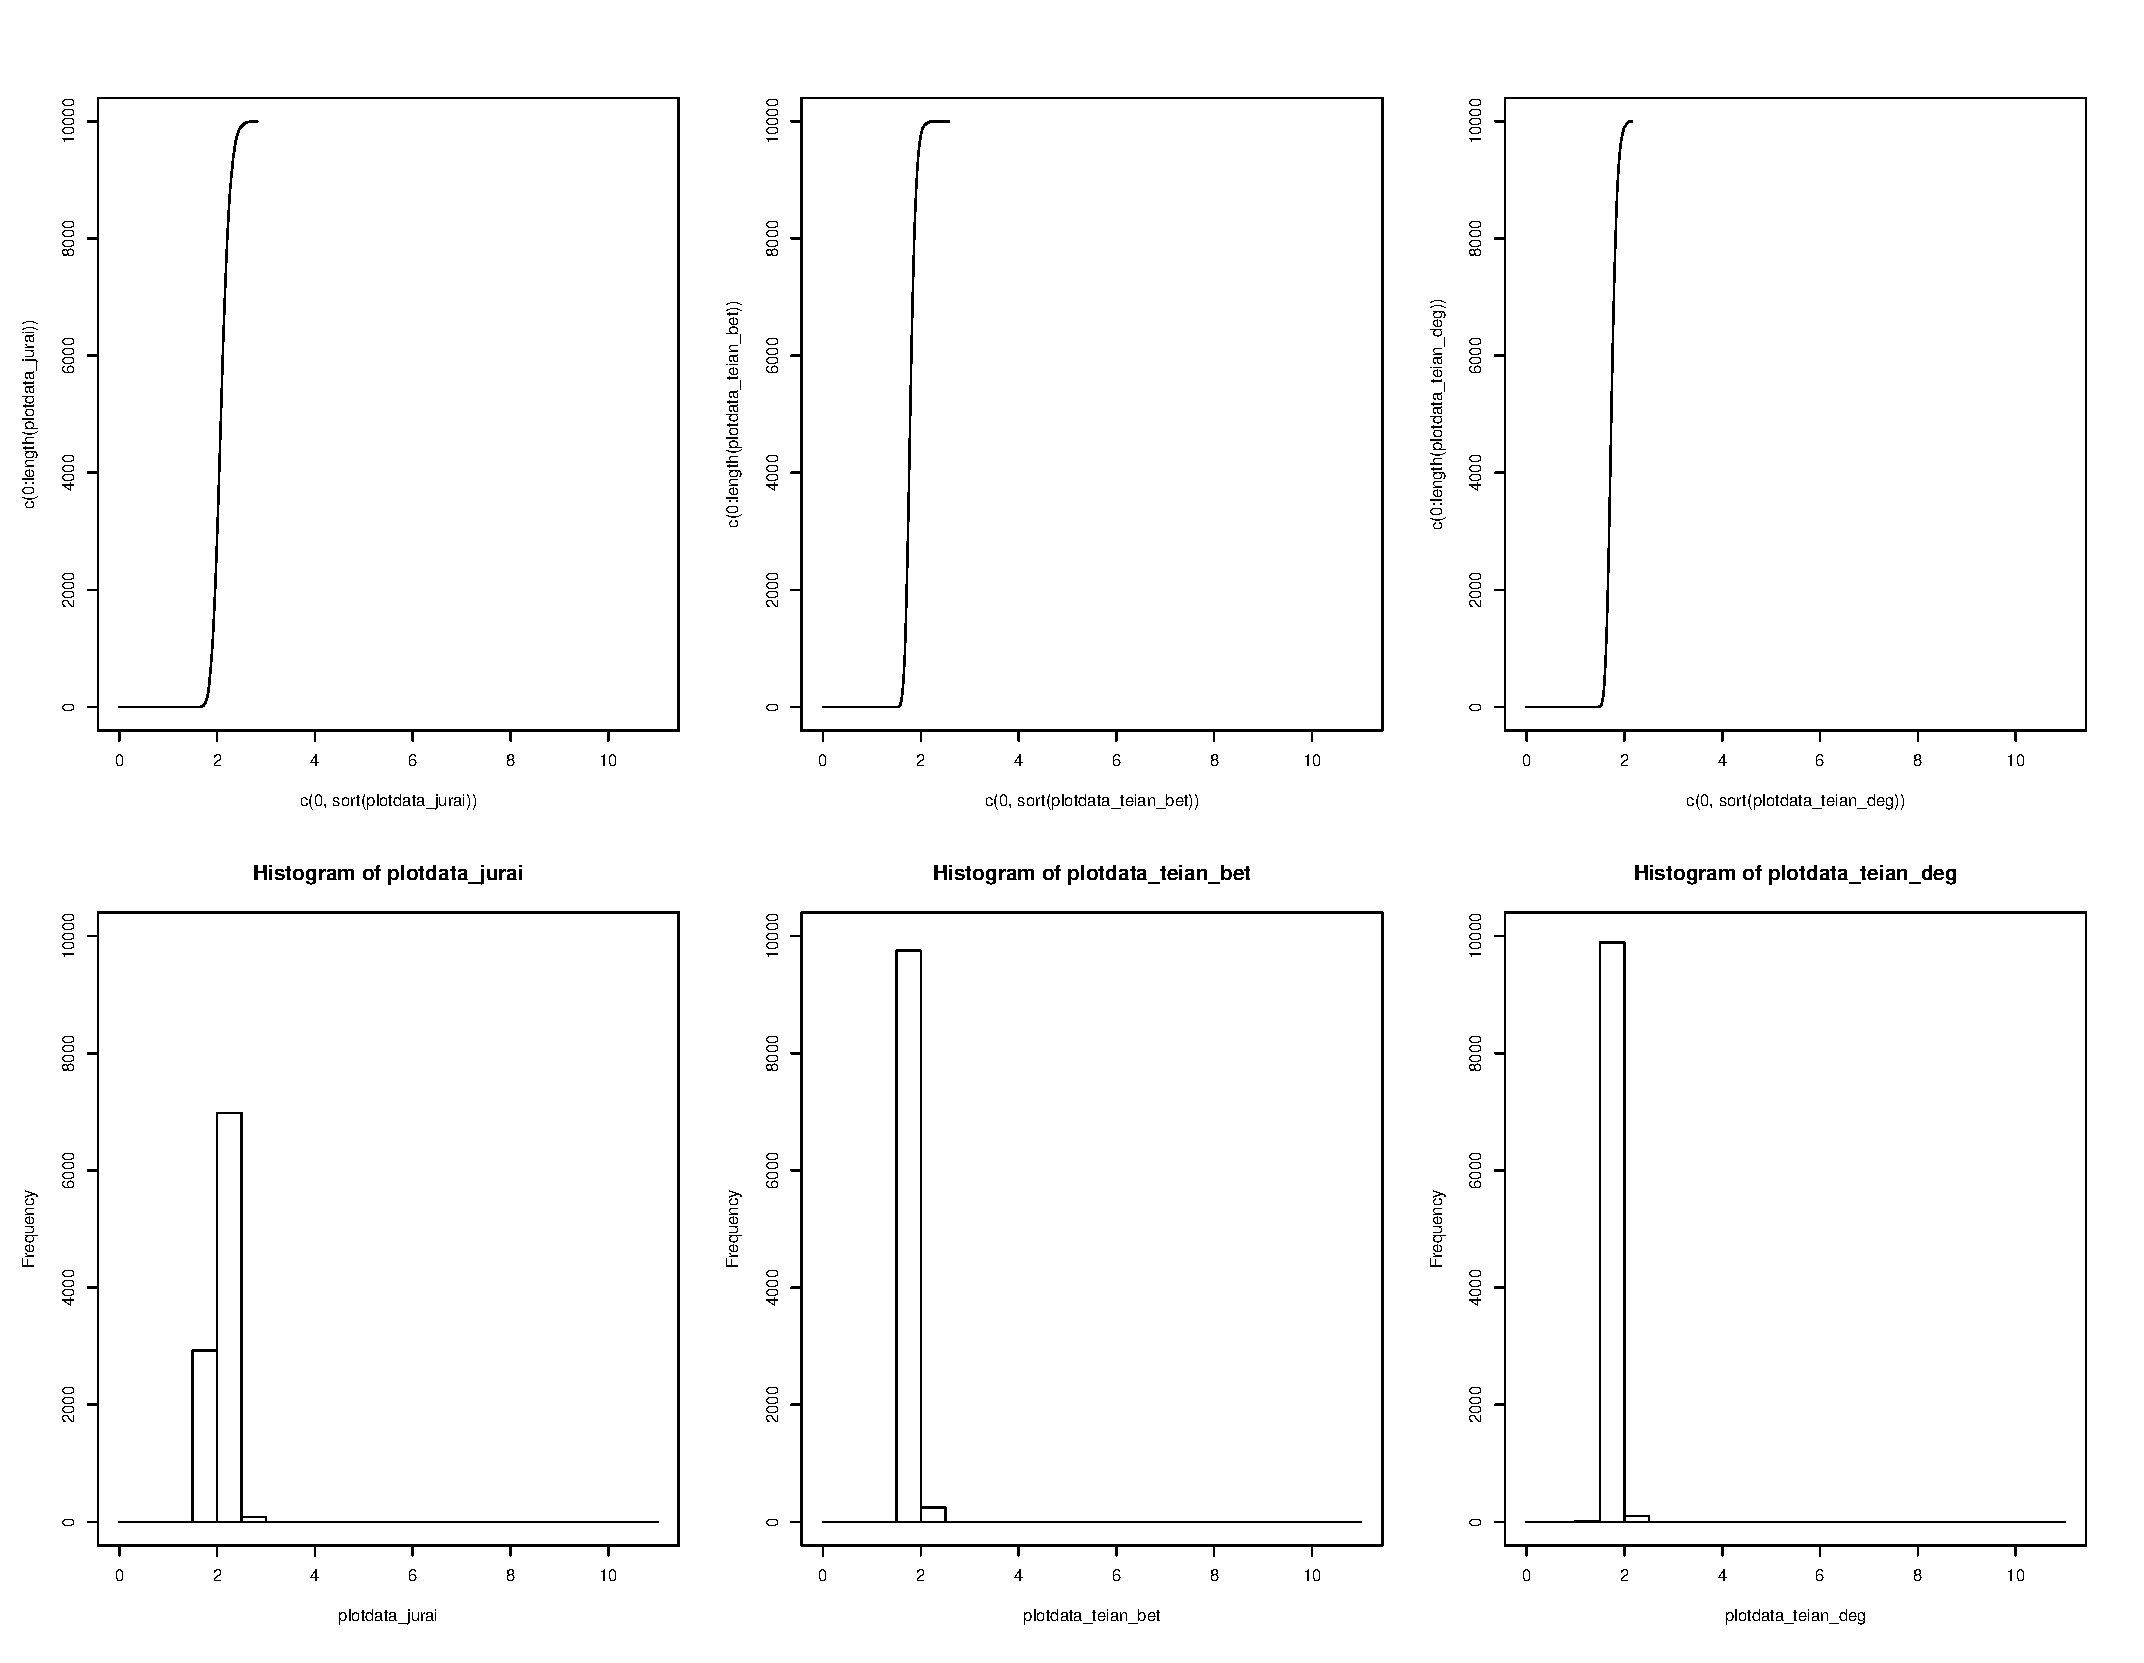
\includegraphics[width=1.2\textwidth]{figures/2_50.eps}
  \caption{方法2:50ノード}
  \label{fig:plot}
\end{figure}

\begin{figure}[H]
  \centering
  \includegraphics[width=1.2\textwidth]{figures/2_100.eps}
  \caption{方法2:100ノード}
  \label{fig:2_100}
\end{figure}
\end{landscape}